\documentclass[letterpaper, 11pt]{article}
\usepackage{epigrafica}%changes default font to epigrafica
\usepackage{comment} % enables the use of multi-line comments (\ifx \fi) 
\usepackage{fullpage} % changes the margin
\usepackage{fancyhdr} % for footer
\usepackage[UKenglish]{isodate}% http://ctan.org/pkg/isodate for date format
\usepackage{wrapfig}
\usepackage[font={small,sf}]{caption}
\usepackage{float}%force tables/figs into certain placement
\usepackage{graphicx}%for figures
\usepackage[]{caption}
\usepackage[leftcaption]{sidecap}%for figure captions
\usepackage{subcaption}%for figures
\usepackage{hyperref}%for hyperlinks
\usepackage[font=small,labelfont=bf]{caption}%for captions
\usepackage{natbib}	%for bibliography
\usepackage{placeins}%prevent images from floating into inappropriate sections
\usepackage{tabulary}%for table at the end, to get soft wrapping
%\usepackage[capbesideposition=inside,facing=yes,capbesidesep=quad]{floatrow}
\usepackage{epigrafica}%changes default font to epigrafica
\usepackage[LGR,OT1]{fontenc}
\newenvironment{labelfontsmall}{\fontfamily{phv}\selectfont}{\par}%for label font example
%\usepackage[T1]{fontenc}

%\captionsetup[figure]{labelformat=empty}% redefines the caption setup of the figures environment in the beamer class.

\def\labelitemi{--}

\pagestyle{fancy}
\renewcommand{\headrulewidth}{0pt}

\lhead{}
\chead{}
\rhead{}
\lfoot{ENT 432 (Fall 2016) - Penn State}
\cfoot{}
\rfoot{\thepage}
\renewcommand{\footrulewidth}{0.4pt}
\title{Collection guidelines: How to prepare, label, and database insect specimens}
\author{Open Entomology Project}

\begin{document}
\cleanlookdateon %removed ordinal date
\maketitle
\thispagestyle{fancy}

\noindent{}The insect collection stands as a core exercise for this course, providing future students and researchers with evidence of your hard work and acquired knowledge and with specimens that serve as vouchers for natural history observations. In this light, proper collecting, specimen preparation, and curation methods are fundamental. This handout provides guidance on current best practices. You may also wish to consult the U.S. Department of Agriculture manual, updated by \cite{USDAmanual}, and other resources for more details regarding the approaches described or alluded to below. 

\section*{Supplies and Equipment}
Some of the equipment needed to observe, collect, and preserve insects will be provided by the instructors. Many of these supplies are also available through vendors like Bioquip (\url{https://www.bioquip.com/}):

\begin{itemize}
\item Vials, 4 dram with polyseal caps (Bioquip \# 8804P)
\item \textgreater70\% ethanol, for preserving insects
\item Shellac (Bioquip \# 1160), for gluing insects to points. You can also use Elmer's or other white glue
\item Points for point mounting (we have point punches and Bristol board for students to use in lab)
\item Stainless steel, size 2 pins (Bioquip \# 1208S2)
\item label paper, 3$\times$5 cards and cellophane envelopes for Odonata
\item Schmitt boxes to store specimens in
\item PSUC identifier labels (a unique number for each specimen)
\item Stereo- and compound microscopes (cannot leave the classroom)
\item Soft-tipped forceps (Bioquip \#'s 4748 or 4750)
\item Waterproof pen for labels; a good option from Bioquip is the size 005 Pigma pen (black) \# 1154E. You can probably find these or their equivalent at an art supply store or even the PSU bookstore
\item ethyl acetate for kill jar
\end{itemize}

\noindent{}Slide-mounting and double-mounting supplies are available upon request, as is acetone for Odonata specimens. These kinds of specimen preparations will be done in the lab.\\

\noindent{}We have collecting equipment that students and members of the Friends of the Frost Entomological Museum can check out for short periods of time; see your instructors. This gear will also be available to everyone during field trips, and sharing is encouraged.

\begin{itemize}
\item UV/Hg-vapor lights with white sheet
\item Yellow bowls
\item Malaise trap
\item Aquatic D net and white pans
\item Winkler extractors, litter sifters
\item Berlese funnel
\item Sweep net
\item Spreading board
\end{itemize}

\noindent{}We can also show you how to make your very own:
 
\begin{itemize}
\item aspirator
\item kill jar
\end{itemize}

\section*{Preparing Hexapoda}
A rough guide to preservation preferences---which taxa are pinned \textit{vs}. slide-mounted, \textit{etc}.---is provided in the Appendix. One should also refer to \cite{USDAmanual} or \cite{USDAmanual1986}.

\paragraph*{Pinning.} Pinning is the best way to preserve hard-bodied, medium to large hexapods. One should use specially made insect pins, rather than common pins used in sewing and other crafts. Insect pins range in size from 000 (VERY thin and mostly unmanageable) to 7 (very thick and longer than most pins). We recommend sizes 1, 2 (especially), and 3 for use in this class. The best way to pin an insect is to:
 
\begin{enumerate}
\item Hold the dead insect between your index finger and thumb
\item Pass the pin vertically through the mesonotum (usually), slightly to the right of center (except in Lepidoptera, which gets the pin through the center of the mesonotum), such that it emerges near the right mid coxa.  Pin placement often varies slightly by taxon (see Figure \ref{pinthorax})
\item Slide the pin far enough through the body such that approximately 1 cm of pin is left between the insect and the pin head (Figure \ref{pinplace}); this forms the ``handle'' for manipulating specimens
\end{enumerate}

\begin{figure}[ht!]
	\centering
  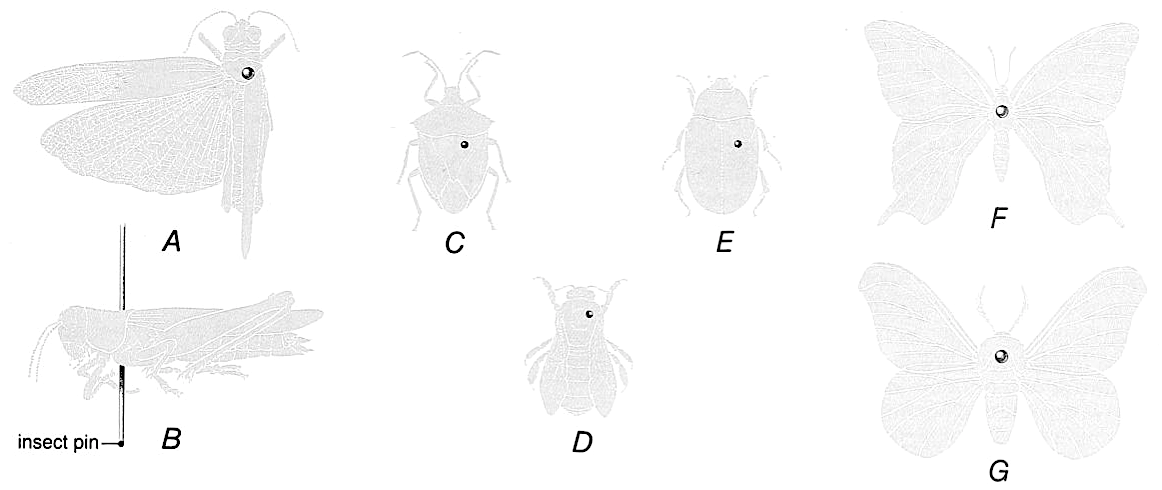
\includegraphics[width=0.75\textwidth]{PinsThorax}
  \caption{Ideal pin placement on different kinds of insects \citep[modified from][Fig. 17]{USDAmanual1986}}
  \label{pinthorax}
\end{figure}

\begin{figure}[ht!]
	\centering
  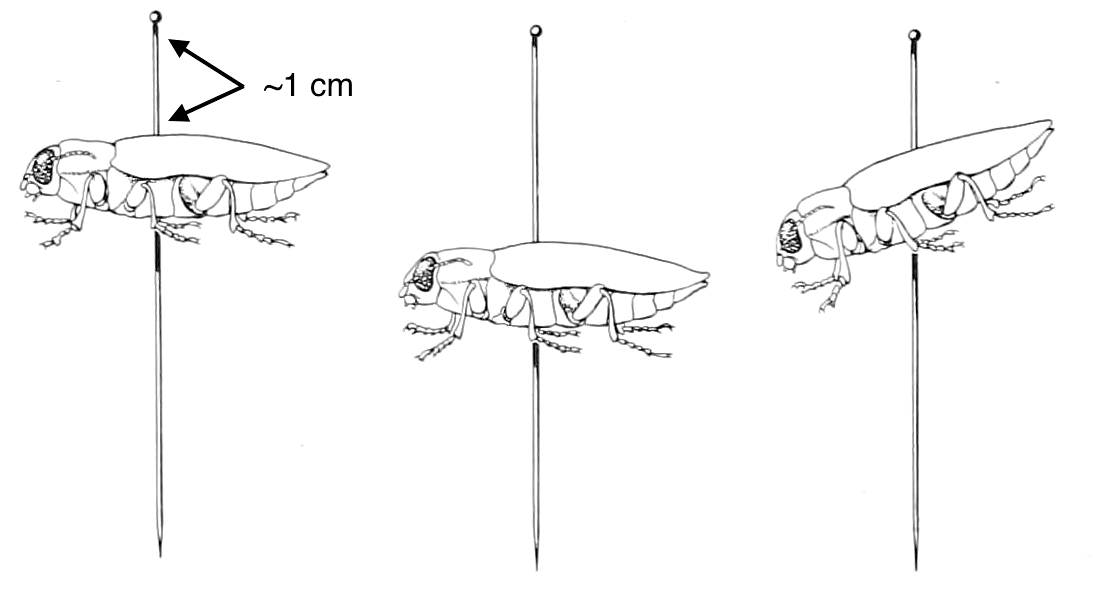
\includegraphics[width=0.55\textwidth]{PinPlacement}
  \caption{Ideal specimen placement on pin (left) and poor placements (middle, right) \citep[modified from][Fig. 16]{USDAmanual1986}}
  \label{pinplace}
\end{figure}

\noindent{}Lepidopterans, especially the larger species, need to have their wings spread by using a spreading board (see Figure \ref{lepspread}). Note that Odonata are never pinned! See Appendix.

\begin{figure}[ht!]
	\centering
  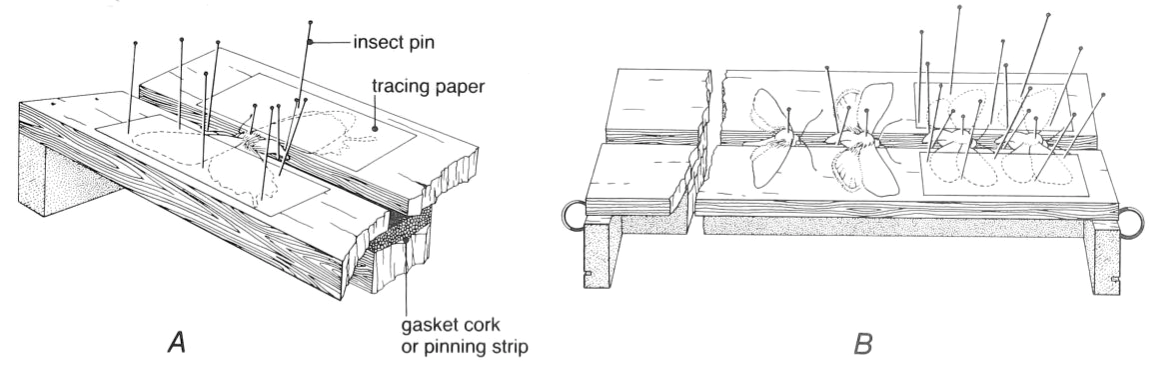
\includegraphics[width=0.85\textwidth]{LepSpreading}
  \caption{How to prepare lepidopteran specimens using a spreading board \citep[][Fig. 20]{USDAmanual1986}}
  \label{lepspread}
\end{figure}

\paragraph*{Pointing.} Smaller insects are usually glued to a triangle (a ``point'') cut or punched from acid-free cardstock or Bristol board. Place a drop of archival glue, such as Gelva, shellac, or polyvinyl acetate (white glue), on the tip of a point that has already been pinned. Touch the point tip to the mesosternum of the insect, usually between the fore and mid coxae. The pointed insect should be oriented in a similar position to that of a pinned insect (Figures \ref{fig:beetlepoint},\ref{fig:flypoint}).\\

\begin{figure}[ht!]
    \centering
    \begin{subfigure}[ht!]{0.43\textwidth}
        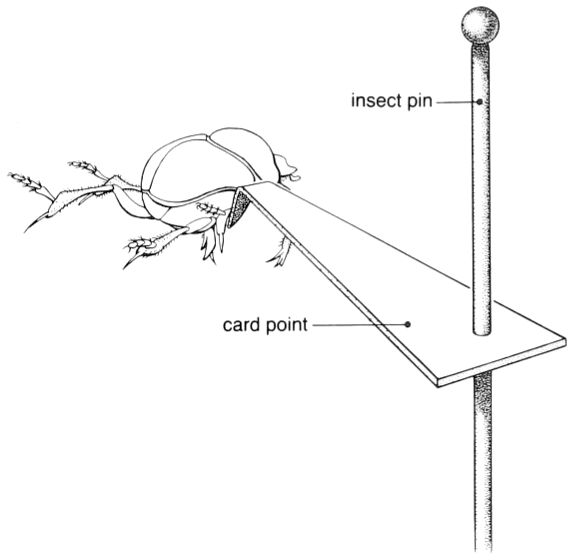
\includegraphics[width=\textwidth]{pointedBeetle}
        \caption{Coleopteran on point \citep[][Fig. 18C]{USDAmanual1986}}
        \label{fig:beetlepoint}
    \end{subfigure}
    \qquad
    \begin{subfigure}[ht!]{0.38\textwidth}
        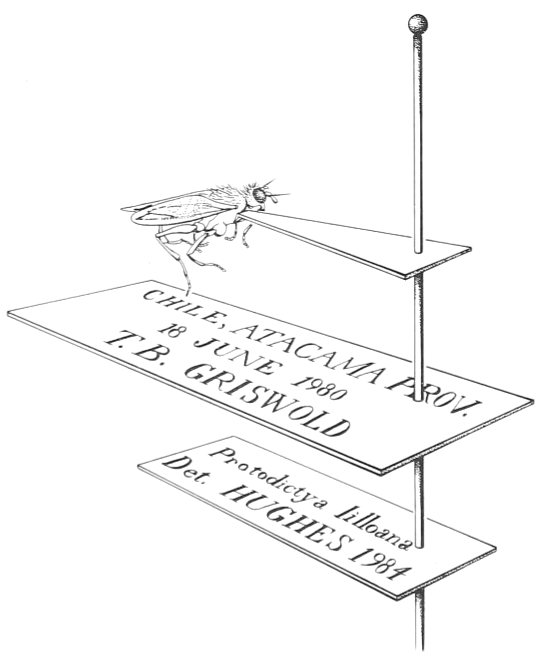
\includegraphics[width=\textwidth]{pointedFly}
        \caption{Dipteran on point \citep[][Fig. 24]{USDAmanual1986}}
        \label{fig:flypoint}
    \end{subfigure}
    \caption{}
\end{figure}

\paragraph*{Double mounts.} Microlepidopterans and scaly flies (\textit{e.g.}, Culicidae) need to be double-mounted using minuten pins. Essentially this is the same as pinning, except one uses a very small pin (the minuten) to mount the specimen. That mount is then affixed to a normal-sized insect pin via a small piece of foam or silicone  (Figures \ref{fig:flymount},\ref{fig:mothmount}). A more detailed description is provided by \cite{GrinterWebpage}.

\begin{figure}[ht!]
    \centering
    \begin{subfigure}[ht!]{0.38\textwidth}
        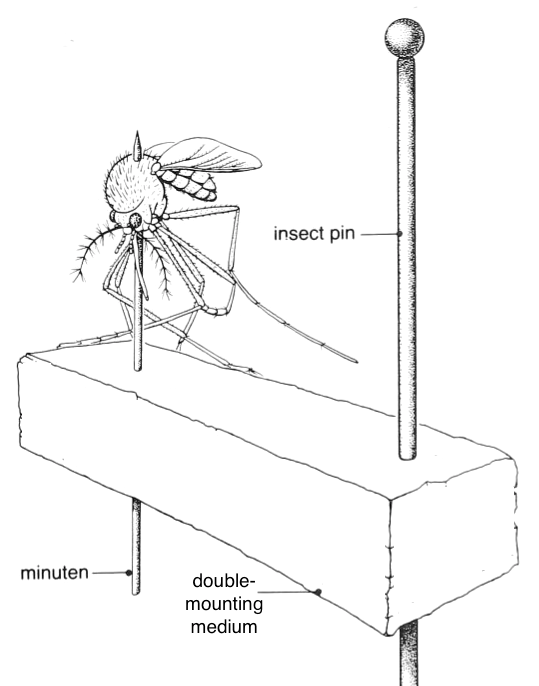
\includegraphics[width=\textwidth]{doublemount}
        \caption{Dipteran on double mount \citep[modified from][Fig. 18A]{USDAmanual1986}}
        \label{fig:flymount}
    \end{subfigure}
    \qquad
    \begin{subfigure}[ht!]{0.42\textwidth}
        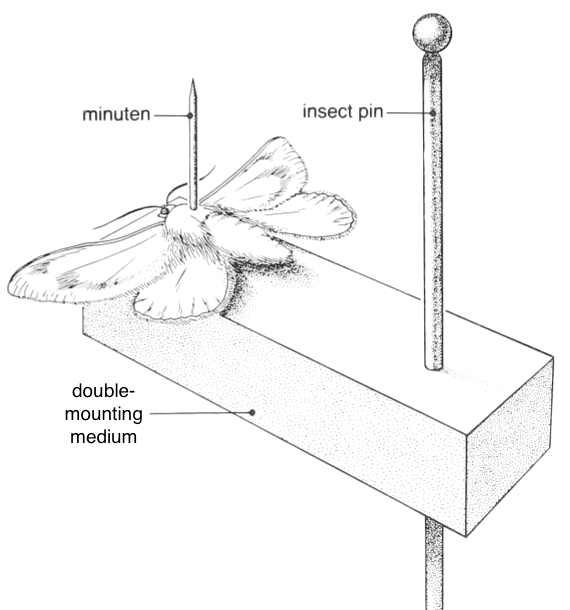
\includegraphics[width=\textwidth]{doublemountMoth}
        \caption{Lepidopteran on double mount \citep[modified from][Fig. 18D]{USDAmanual1986}; this specimen is arguably too close to the medium but is oriented correctly}
        \label{fig:mothmount}
    \end{subfigure}
    \caption{}
\end{figure}

\paragraph*{Alcohol.} Soft-bodied hexapods, including all immature stages and aquatic insects (except perhaps Coleoptera), must be preserved in alcohol, rather than being pinned or pointed. Hexapods preserved in \textgreater95\% alcohol are best for DNA extraction, especially if they are kept cold. Unfortunately, high concentrations of alcohol also tend to make specimens a bit fragile, by dehydrating them. Concentrations below 70\% are generally not recommended, as specimens have a better chance of rotting. We use 70--80\% ethanol in the lab, which works well for nearly any kind of hexapod. Adult Lepidoptera should never be preserved in ethanol, as the scales will detach.

\paragraph*{Slide Mounting.} Slide-mounted preparations are critical for proper diagnosis of certain taxa, especially small insects. The methods are typically intensive and so are beyond the scope of this course. See \cite{SlideMounting} for the methods and justification if you're interested.

\section*{Locality Labels}
Labels can take many forms, but you generally want to adhere to the following formats:

\begin{enumerate}
\item Labels always begin with the country (sometimes in \textbf{bold} or ALL CAPS) and continue with finer scale details of the locality. One should always include the latitude and longitude---using decimal based degrees is preferred over minutes and/or seconds, as they are easier to database.
\item The date should be formatted such that the month is in lowercase Roman numerals (\textit{e.g.}, October would be ``x''): 12.x.2010 or 11--12.x.2010 or 11.x--12.xi.2010
\item The collector's name(s) should also be included, as should the collecting method. Common abbreviations include: MT = Malaise trap, YPT = yellow pan trap, FIT = flight intercept trap, SS = screen sweep. Collectors' names are sometimes followed by ``leg.'', which is short for the Latin ``lego'', to gather or collect.
\item A sans-serif font (like Arial Narrow) makes the label more readable when the size gets small. Most people use 4 pt for the font size. The finished label should be informative, with a minimal amount of abbreviations, but also reasonably small in size. The information should also be presented in a symmetrical label that minimizes white space:\\

\begin{labelfontsmall}
\tiny 
\noindent{USA: PA: Centre County: \\ Pine Grove Mills, 40.730, \\ -77.884, $\pm$ 250m 15.iv.2016 \\ A.R. Deans, sifted litter}
\end{labelfontsmall}
\normalsize

\item Labels that seem to be excessively large can be cut into two labels. Specimens are prone to multiple labeling from future studies (voucher label, determination label, accession numbers, barcodes, \textit{etc.}), so it's desirable to keep the label number to a minimum.
\item Use cotton rag, acid free cardstock for printing labels.
\end{enumerate}

\section*{Fluid-preserved Specimens}%fix this; integrate with above
Same suggestions apply to labels for fluid-preserved specimens, but one can and should make his/her labels slightly larger (maybe 6 pt) and more elongate:\\

\hfill\begin{minipage}{\dimexpr\textwidth-1cm}
\begin{labelfontsmall}
\scriptsize 
\noindent{USA: PA: Centre County: Pine Grove Mills\\ Slab Cabin Run, 40.730, -77.884, $\pm$ 250m \\hand collected off rocks, 15.iv.2016 A.R. Deans}
\end{labelfontsmall}
\xdef\tpd{\the\prevdepth}
\end{minipage}
\normalsize\vspace{5mm}

\noindent{}Small labels act like blades and chop up wet-preserved specimens, which are usually relatively soft-bodied.

\section*{Determination Labels}
Determination (``det'') labels can also vary in their appearance, but it's important that they include the taxon name(s), the name of the determiner, and the year (or date) the determination was made. Again, det labels for fluid preserved specimens should be slightly larger and more elongate.\\

\hfill\begin{minipage}{\dimexpr\textwidth-1cm}
\begin{labelfontsmall}
\tiny 
\noindent{Hymenoptera:\\ Megaspilidae\\ det. A.R. Deans 2016}
\end{labelfontsmall}
\xdef\tpd{\the\prevdepth}
\end{minipage}
\normalsize\vspace{2mm}


\section*{Shipping specimens}
Once prepared it is not unusual to ship specimens to experts for diagnosis or to museums to be deposited for perpetuity. We won't be shipping anything as part of this course, but if you need to ship specimens in the future see \cite{packinginsects} and \cite{MacraeWebpage}.

\FloatBarrier
% adding bibliography here
\bibliographystyle{apalike}
\bibliography{bib}

\clearpage
\section*{Appendix. Insect collection and preservation guide}
The table below should not be considered as the definitive guide to insect preservation but rather as a quick reference for how these insects are typically preserved---\textit{i.e.}, a ``What can I do now that I caught this hexapod?'' guide. Note that the original photos below were accessed on 1 August 2016. Please notify the Project of errors by using the GitHub issue tracker:\\ \url{https://github.com/OpenEntomology/InsectBiodiversityEvolution/issues}

\begin{SCfigure}[][ht!]
  \caption*{\textbf{Entognatha} (proturans, diplurans, springtails). \textit{Habitat:} leaf litter, under rocks/logs. \textit{Collecting method:} Winkler extractor, Berlese funnel. \textit{How to euthanize:} Submerge in ethanol. \textit{Prepare specimens:} Traditionally slide-mounted, but for this class they can be stored in vials with ethanol (\textgreater70\%) as the preservative.\\ Photo: Andy Murray (CC BY-SA 2.0) \url{https://flic.kr/p/bJCR9e}}
  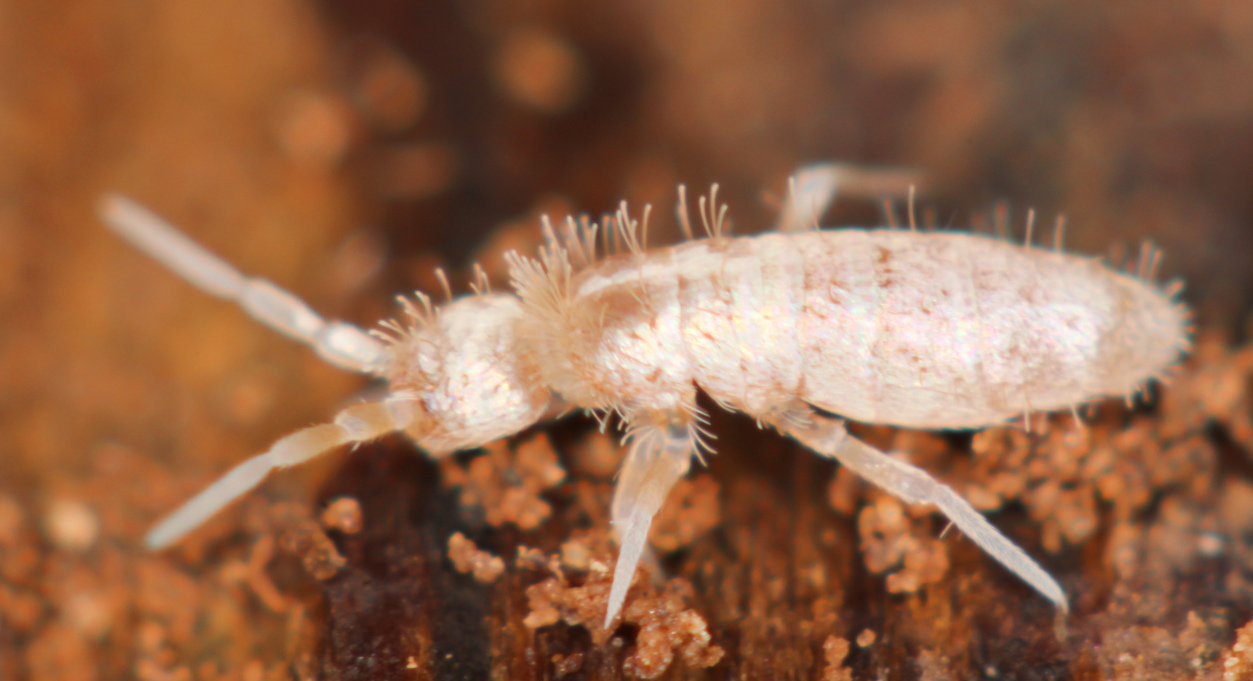
\includegraphics[width=0.45\textwidth]{Collembola}
\end{SCfigure}

\begin{SCfigure}[][ht!]
  \caption*{\textbf{Archaeognatha} (bristletails). \textit{Habitat:} leaf litter, inside buildings. \textit{Collecting method:} Aspirator, forceps. \textit{How to euthanize:} Submerge in ethanol. \textit{Prepare specimens:} Preserve in vials with ethanol (\textgreater70\%).\\ Photo: Henry Lydecker (CC BY-NC 2.0) \url{https://flic.kr/p/dgRtaW}}
  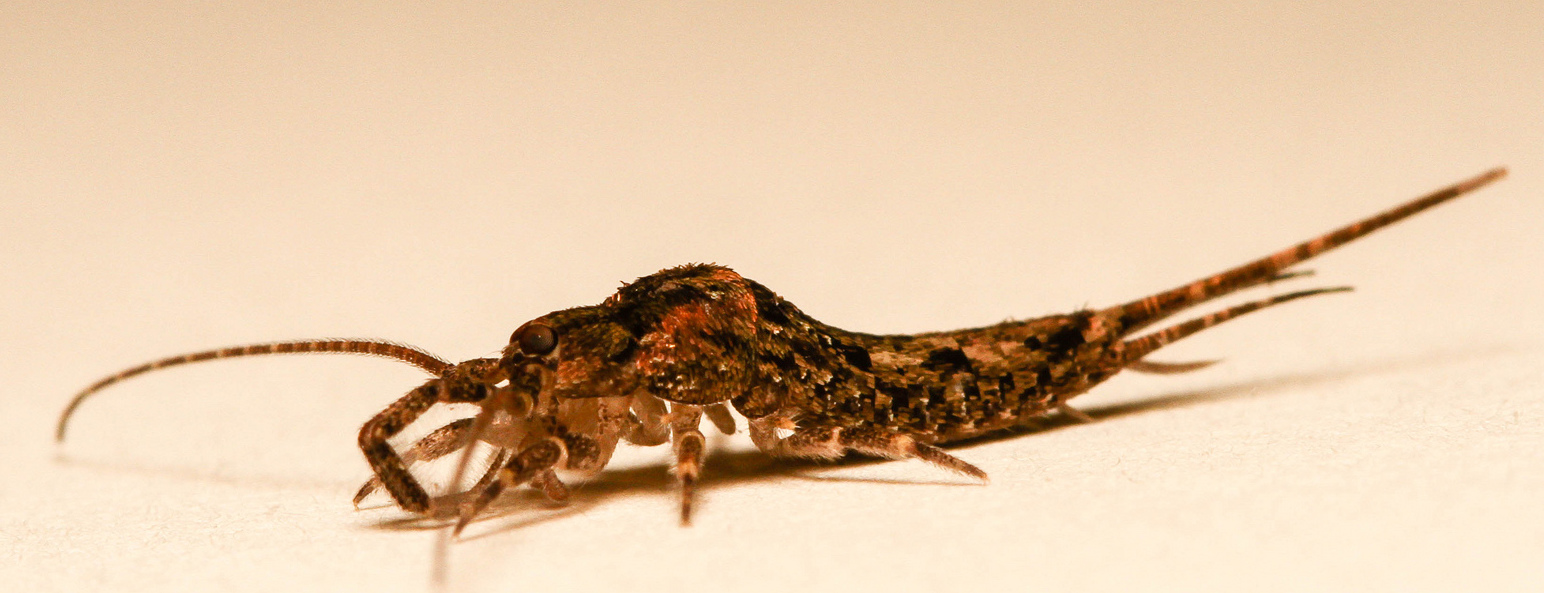
\includegraphics[width=0.45\textwidth]{Archeognatha}
\end{SCfigure}

\begin{SCfigure}[][ht!]
  \caption*{\textbf{Zygentoma} (silverfish, firebrats). \textit{Habitat:} leaf litter, on logs at night. \textit{Collecting method:} Aspirator, net. \textit{How to euthanize:} Submerge in ethanol. \textit{Prepare specimens:} Preserve in vials with ethanol (\textgreater70\%).\\ Photo: Jean-Rapha\"{e}l Guillaumin (CC BY-SA 2.0) \url{https://flic.kr/p/czibHd}}
  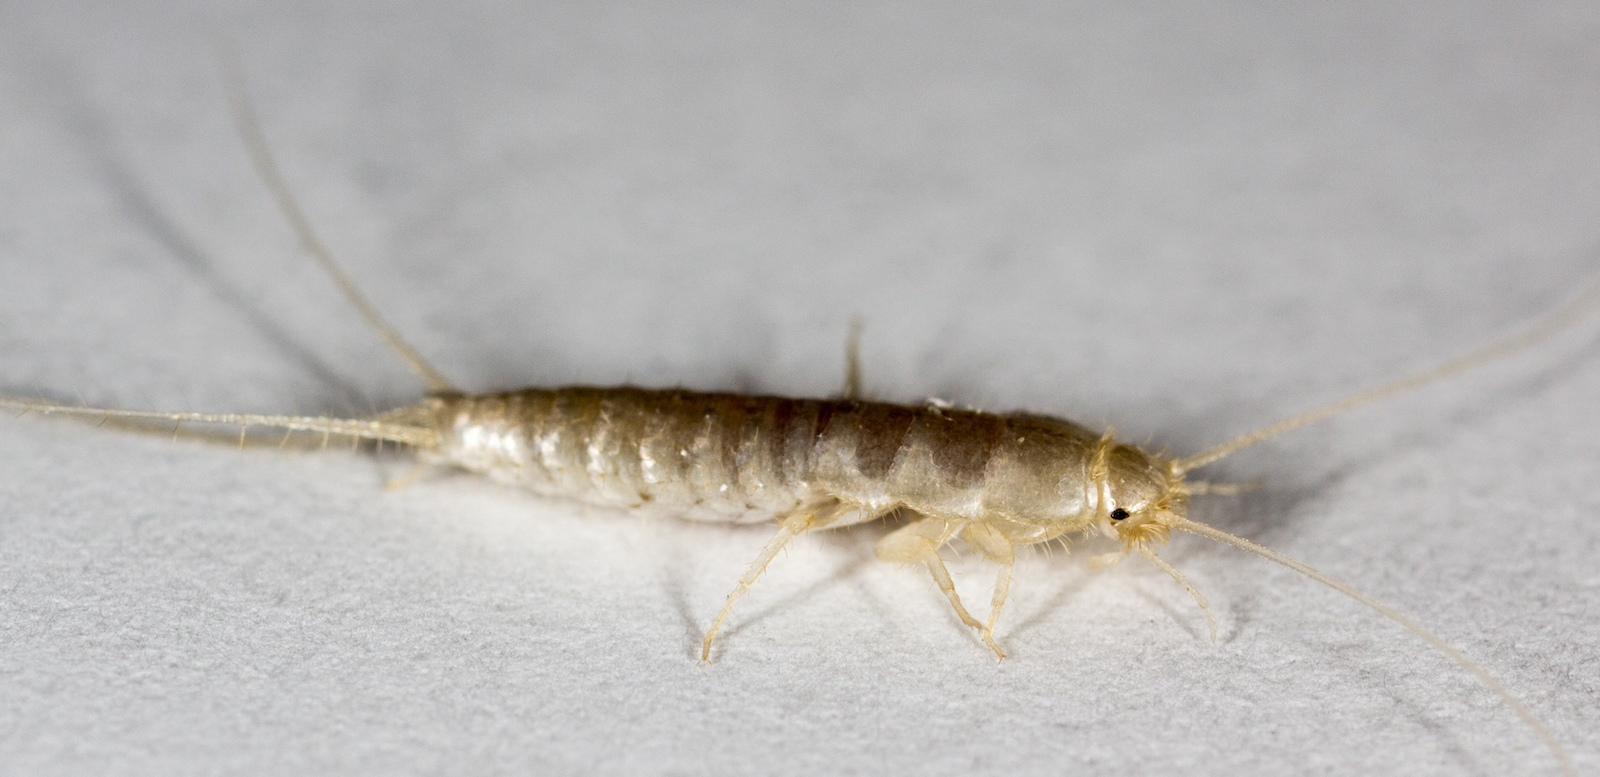
\includegraphics[width=0.45\textwidth]{Zygentoma}
\end{SCfigure}

\begin{SCfigure}[][ht!]
  \caption*{\textbf{Ephemeroptera} (mayflies). \textit{Habitat:} Immatures are aquatic; adults fly. \textit{Collecting method:} Use D-net for immatures; aspirator, net, and/or sheet at light for adults. \textit{How to euthanize:} Submerge in ethanol. \textit{Prepare specimens:} Preserve all stages in vials with ethanol (\textgreater70\%); note that these specimens will be fragile!\\ Photo: Magnus Hagdorn (CC BY-SA 2.0) \url{https://flic.kr/p/ffsx8c}}
  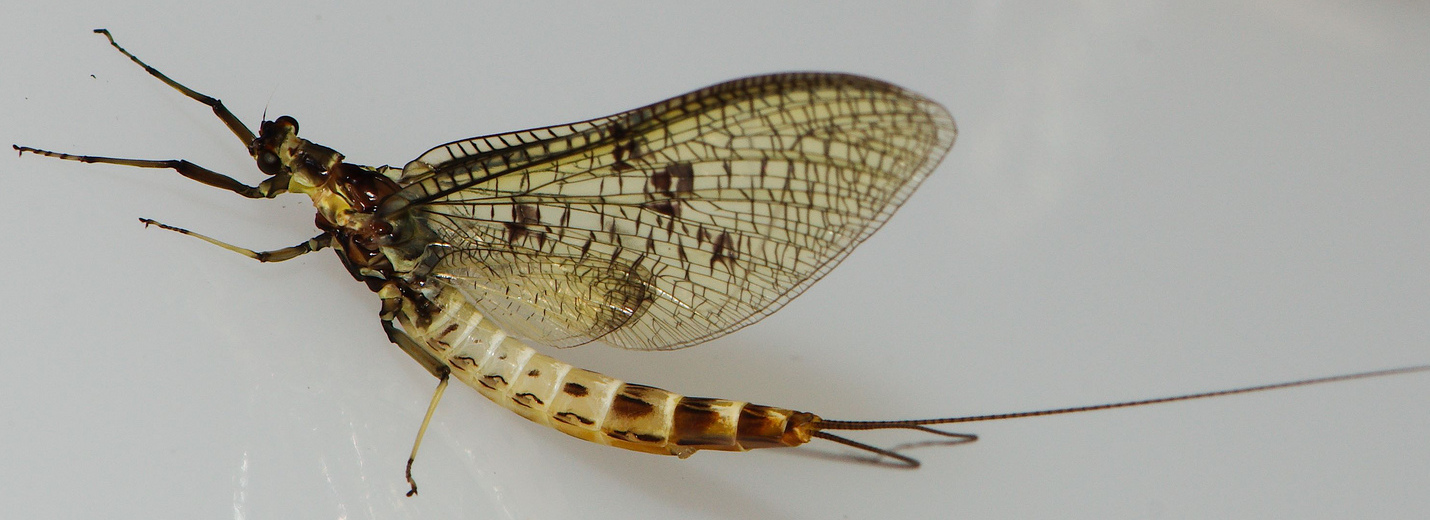
\includegraphics[width=0.45\textwidth]{Ephemeroptera}
\end{SCfigure}

\clearpage

\begin{SCfigure}[][ht!]
  \caption*{\textbf{Odonata} (dragonflies and damselflies). \textit{Habitat:} Immatures are aquatic; adults fly. \textit{Collecting method:} Use D-net for immatures, aerial net for adults. \textit{How to euthanize:} Adults should be kept alive in glassine envelope or paper triangle until they can be euthanized by submersion in acetone. Larvae are euthanized in ethanol, like other insects. \textit{Prepare specimens:} Soak in acetone overnight, then let air dry. Dried specimens are preserved with a 3$\times$5 card (with locality label), inside a cellophane envelope. Larvae are always preserved in vials with ethanol (\textgreater70\%).\\ Photo: Andy Deans (CC BY 2.0) \url{https://flic.kr/p/oa95N7}}
  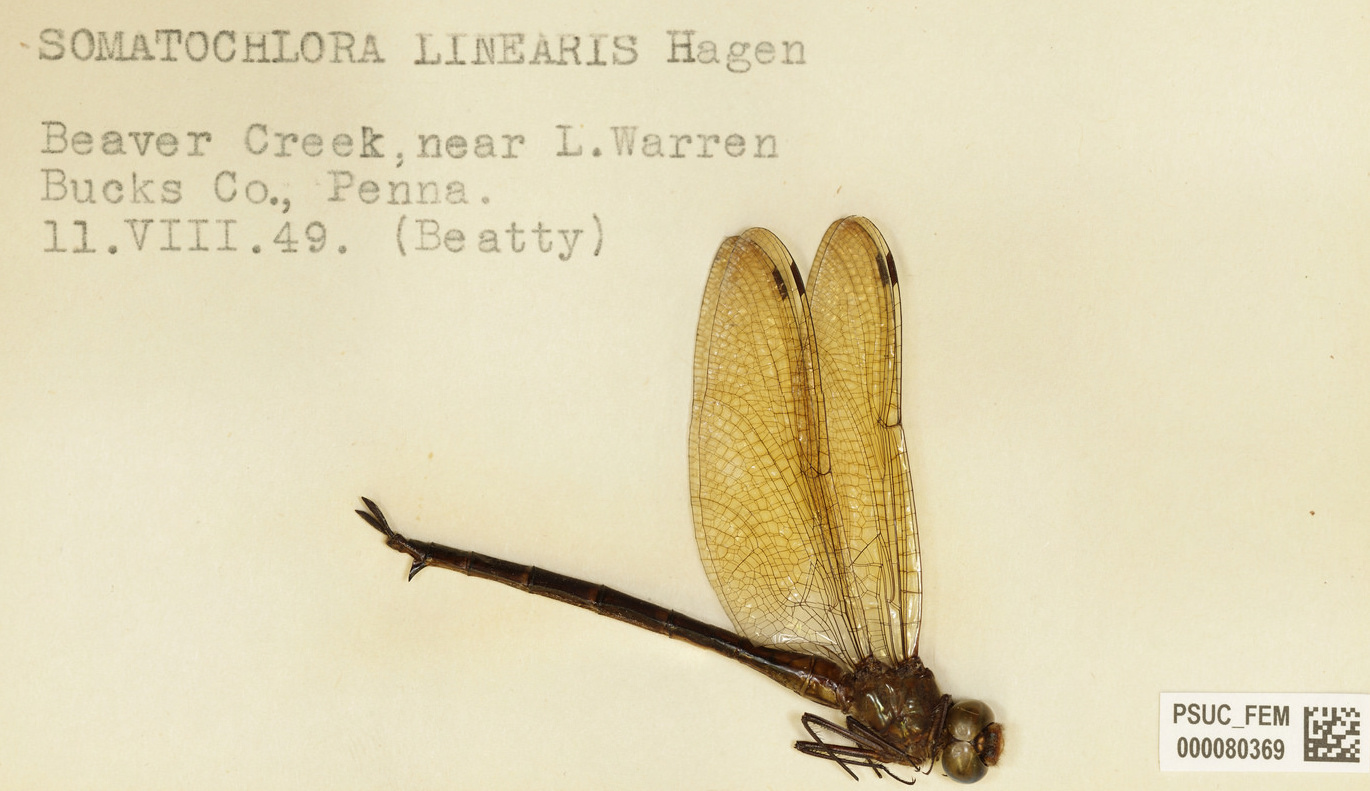
\includegraphics[width=0.45\textwidth]{Odonata}
  \label{odonataprep}
\end{SCfigure}

\begin{SCfigure}[][ht!]
  \caption*{\textbf{Phasmatodea} (walking stick, stick insects, leaf insects). \textit{Habitat:} Trees, fence posts. \textit{Collecting method:} By hand, net. \textit{How to euthanize:} Freeze or use kill jar with ethyl acetate. \textit{Prepare specimens:} Nymphs are preserved in vials with ethanol (\textgreater70\%). Adults are pinned through mesothorax, with legs, wings (if present) and antennae pinned near body to minimize overall specimen size. \\ Photo: Norman Walsh (CC BY-NC 2.0) \url{https://flic.kr/p/3gcGh5}}
  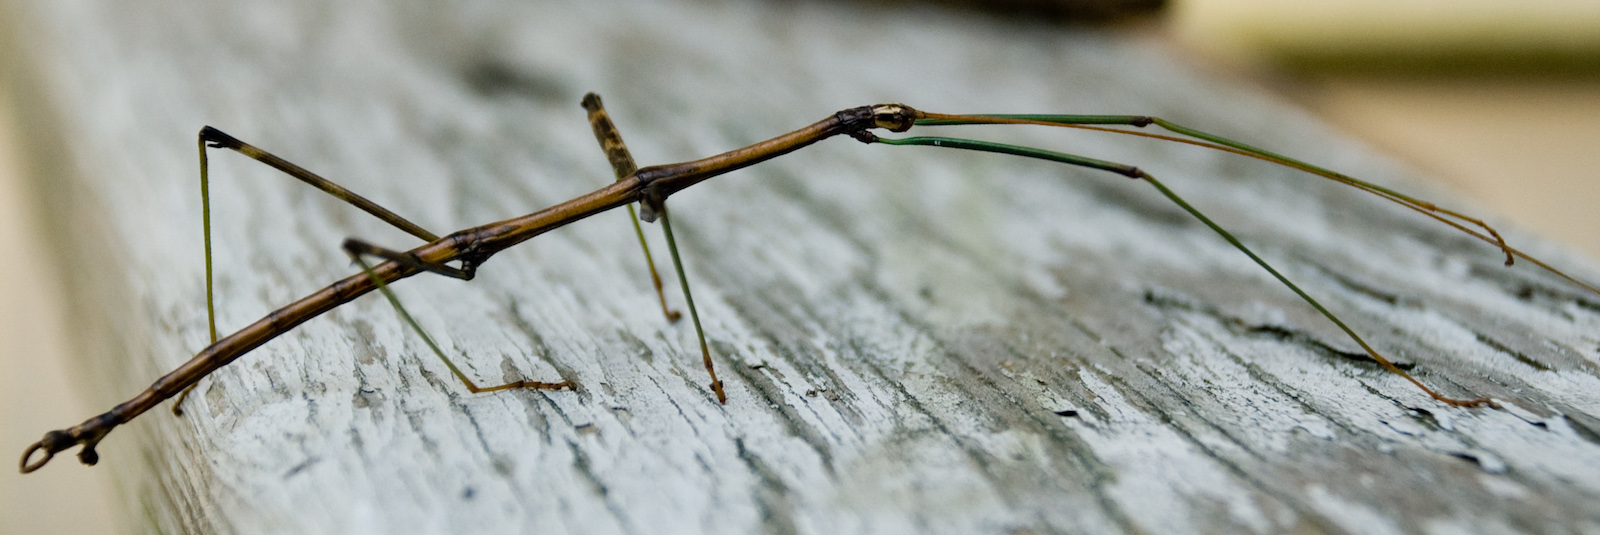
\includegraphics[width=0.45\textwidth]{Phasmatodea}
\end{SCfigure}

\begin{SCfigure}[][ht!]
  \caption*{\textbf{Orthoptera} (grasshoppers, crickets, katydids). \textit{Habitat:} Grasses, trees, shrubs. \textit{Collecting method:} By hand, net, with baits. \textit{How to euthanize:} Freeze or use kill jar with ethyl acetate. \textit{Prepare specimens:} Nymphs and soft-bodied taxa (\textit{e.g.}, Gryllidae) are preserved in vials with ethanol (\textgreater70\%). Adults are pinned through mesothorax, with legs and antennae pinned near body to minimize overall specimen size. Note that the guts of large specimens should be removed prior to pinning (insert sharp forceps under the posterior edge of pronotum, grab gut and pull out). Left wings could be spread. \\ Photo: Andreas Kay (CC BY-NC-SA 2.0) \url{https://flic.kr/p/mR5QLa}}
  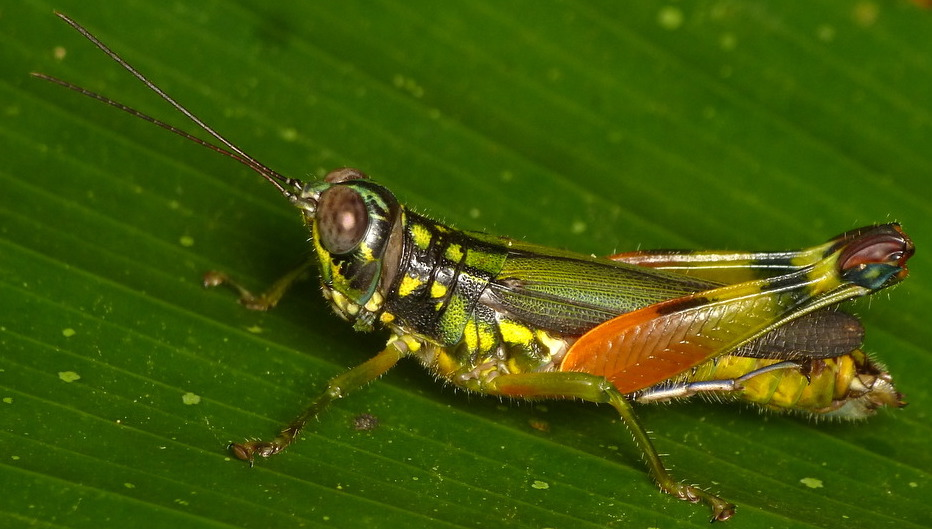
\includegraphics[width=0.45\textwidth]{Orthoptera}
\end{SCfigure}

\clearpage

\begin{SCfigure}[][ht!]
  \caption*{\textbf{Grylloblattodea}. \textit{Habitat:} Snow pack, glaciers of western North America. \textit{Collecting method:} By hand. \textit{How to euthanize:} Submerge in ethanol. \textit{Prepare specimens:} Preserve in vials with ethanol (\textgreater70\%).\\ Photo: Alex Wild (CC0) \url{https://goo.gl/DAU1HJ} (Wikimedia Commons)}
  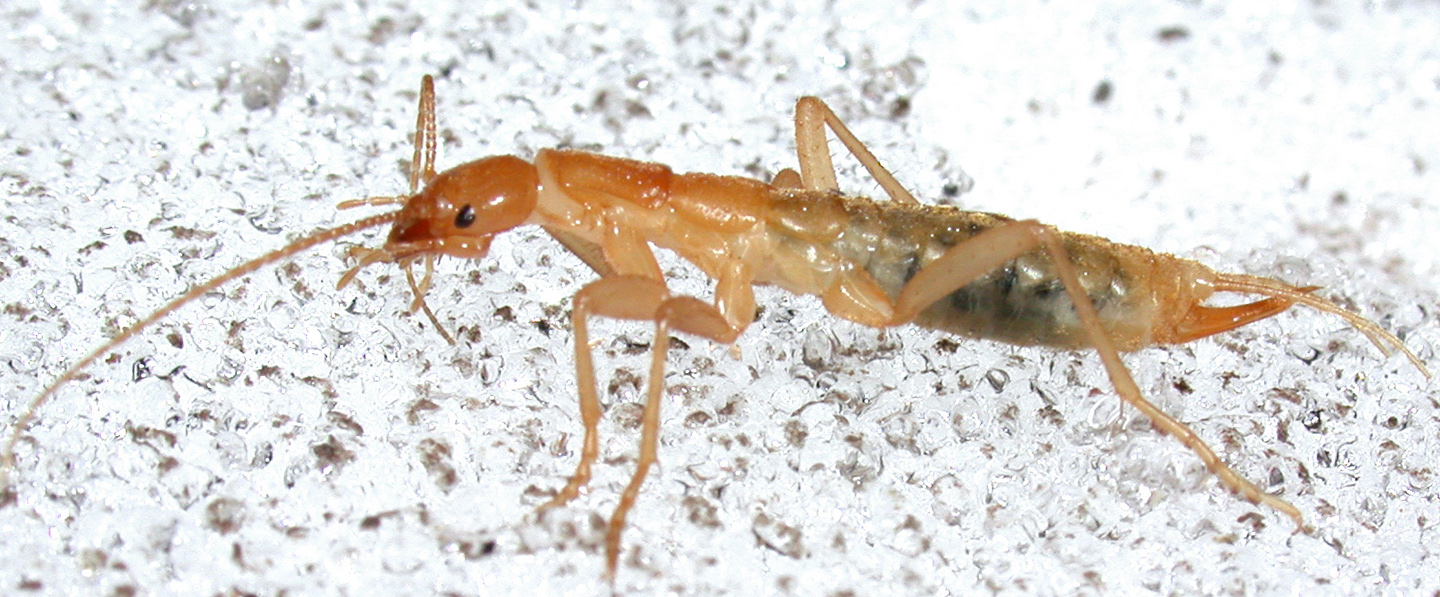
\includegraphics[width=0.45\textwidth]{Grylloblattodea}
\end{SCfigure}

\begin{SCfigure}[][ht!]
  \caption*{\textbf{Mantophasmatodea}. \textit{Habitat:} Grasses, shrubs, and rocks of southern Africa. \textit{Collecting method:} By hand. \textit{How to euthanize:} Freeze or submerge in ethanol. \textit{Prepare specimens:} Preserve in vials with ethanol (\textgreater70\%).\\ Photo: P. E. Bragg (CC BY-SA 3.0) \url{https://goo.gl/kpnn99} (Wikimedia Commons)}
  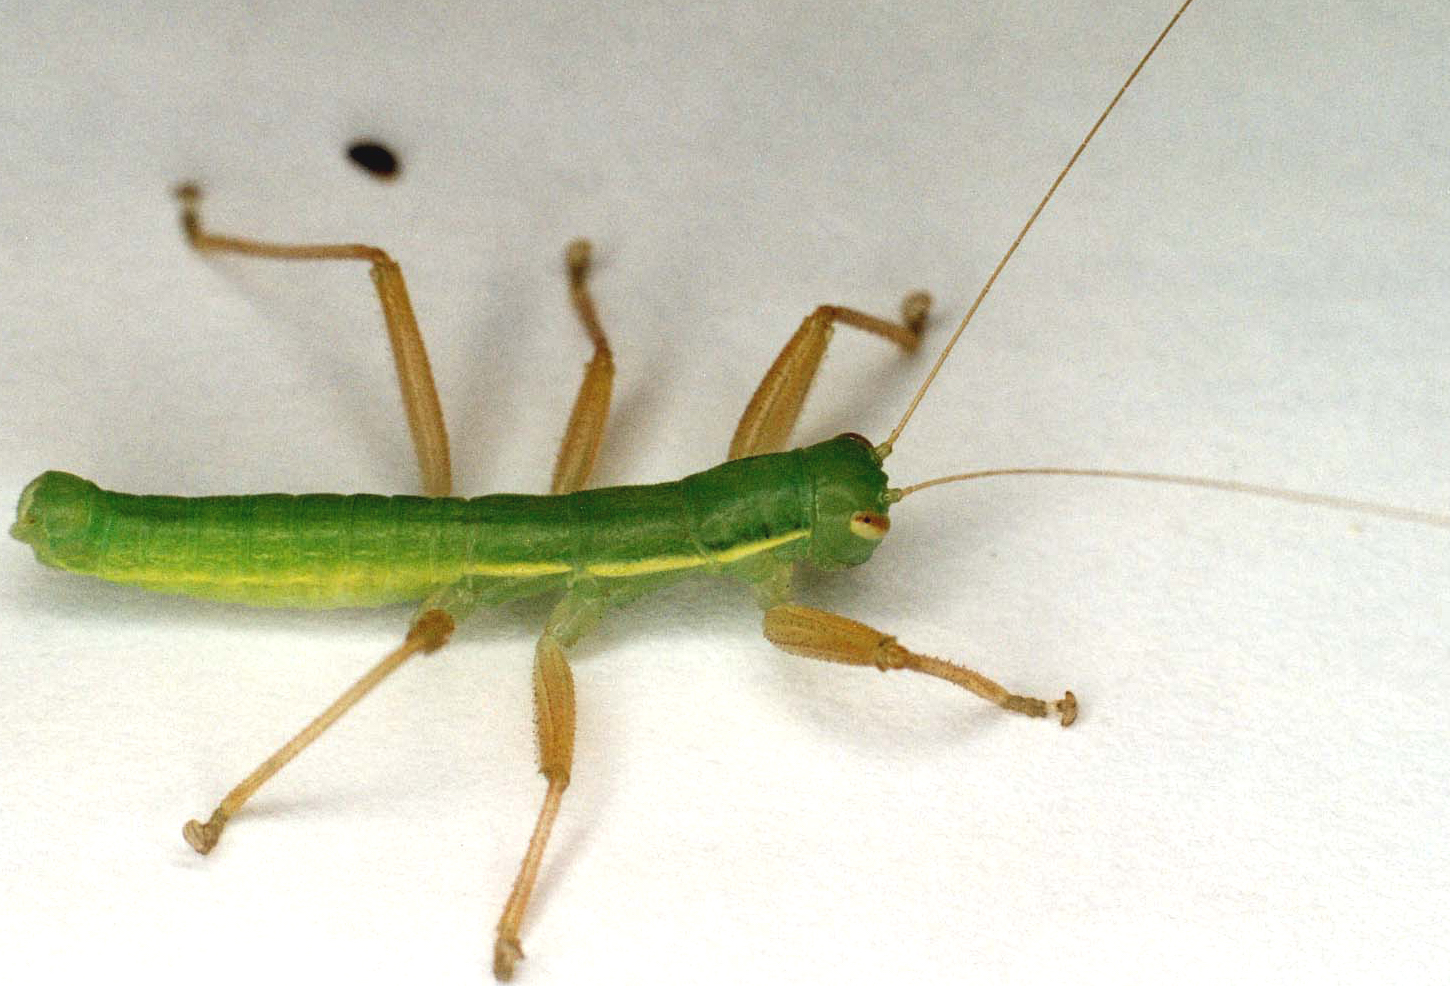
\includegraphics[width=0.45\textwidth]{Mantophasmatodea}
\end{SCfigure}

\begin{SCfigure}[][ht!]
  \caption*{\textbf{Dermaptera} (earwigs). \textit{Habitat:} Under rocks and logs. \textit{Collecting method:} By hand, on sheet at light. \textit{How to euthanize:} Freeze, submerge in ethanol, or use kill jar with ethyl acetate. \textit{Prepare specimens:} Pin through mesothorax.\\ Photo: Mick E. Talbot (CC BY-NC-SA 2.0) \url{https://flic.kr/p/baT4zp}}
  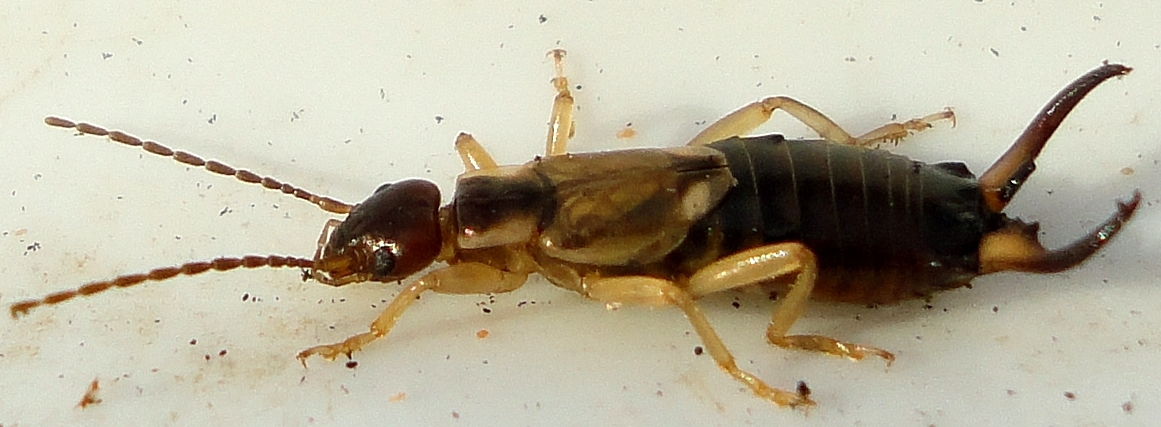
\includegraphics[width=0.45\textwidth]{Dermaptera}
\end{SCfigure}

\begin{SCfigure}[][h!]
  \caption*{\textbf{Non-isopteran Dictyoptera} (cockroaches, mantids). \textit{Habitat:} Under rocks and logs; also inside buildings. \textit{Collecting method:} By hand, on sheet at light. \textit{How to euthanize:} Freeze, submerge in ethanol, or use kill jar with ethyl acetate. \textit{Prepare specimens:} Pin through mesothorax and keep appendages close to body; male genitalia are useful for species-level diagnosis, so maximize their visibility.\\Photo: Martin Grimm (CC BY-NC-SA 2.0) \url{https://flic.kr/p/aVJPH8}}
  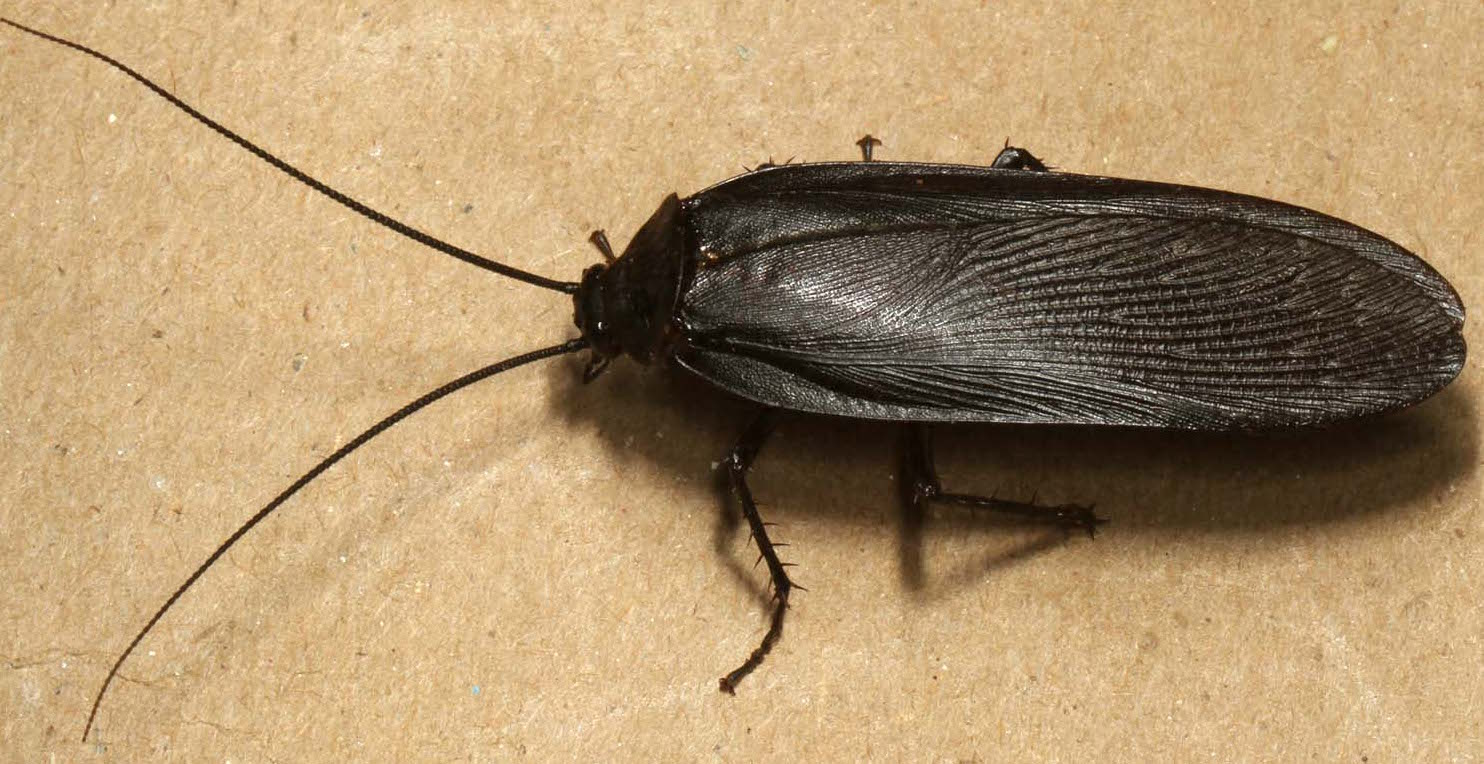
\includegraphics[width=0.45\textwidth]{Blattodea}
\end{SCfigure}

\clearpage

\begin{SCfigure}[][ht!]
  \caption*{\textbf{Dictyoptera: Isoptera} (termites). \textit{Habitat:} Under rocks and logs; also inside buildings. \textit{Collecting method:} By hand, with aspirator, with net, on sheet at light. \textit{How to euthanize:} Submerge in ethanol. \textit{Prepare specimens:} Preserve in vials with ethanol (\textgreater70\%). \\ Photo: Stevenw12339 (CC BY-NC 2.0) \url{https://flic.kr/p/fAdvLc}}
  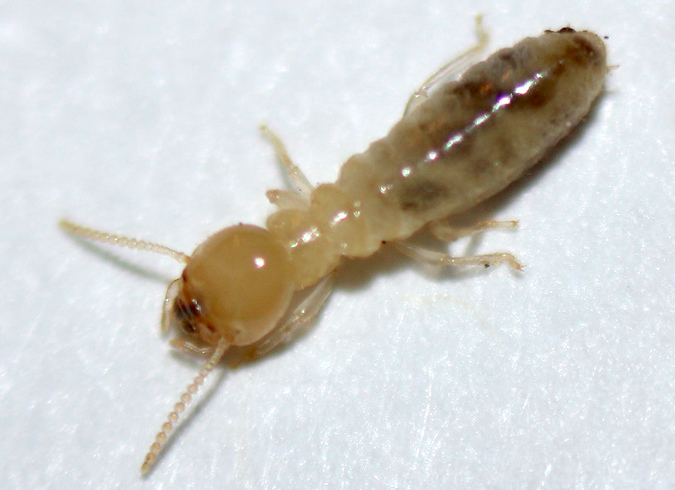
\includegraphics[width=0.45\textwidth]{BlattodeaIsoptera}
\end{SCfigure}

\begin{SCfigure}[][ht!]
  \caption*{\textbf{Embioptera} (webspinners). \textit{Habitat:} Under rocks and logs, on tree trunks. \textit{Collecting method:} Look for silken galleries and collect by hand; may also come to lights. \textit{How to euthanize:} Submerge in ethanol. \textit{Prepare specimens:} Preserve in vials with ethanol (\textgreater70\%).\\ Photo: Bill \& Mark Bell (CC BY-NC-SA 2.0) \url{https://flic.kr/p/cCJB7S}}
  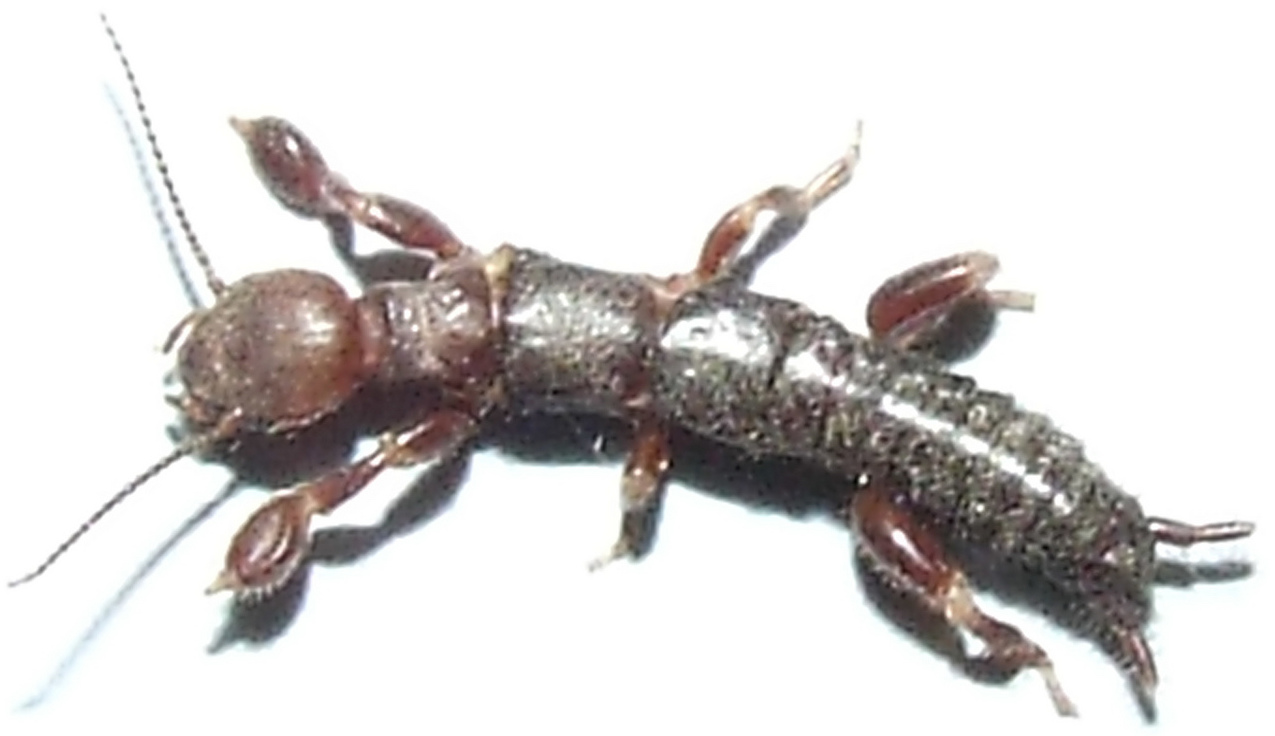
\includegraphics[width=0.45\textwidth]{Embioptera}
\end{SCfigure}

\begin{SCfigure}[][ht!]
  \caption*{\textbf{Zoraptera}. \textit{Habitat:} Under logs, especially in or near sawdust. \textit{Collecting method:} By hand or with Winkler extractor or Berlese funnel. \textit{How to euthanize:} Submerge in ethanol. \textit{Prepare specimens:} Preserve in vials with ethanol (\textgreater70\%).\\ Photo: David Maddison (CC BY 3.0) \url{http://goo.gl/hSP3EW} (tolweb.org)}
  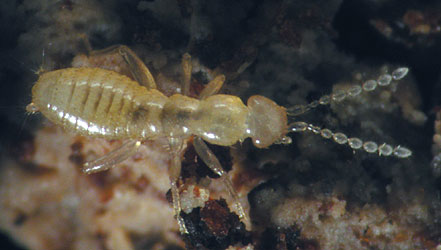
\includegraphics[width=0.45\textwidth]{Zoraptera}
\end{SCfigure}

\begin{SCfigure}[][ht!]
  \caption*{\textbf{Plecoptera} (stoneflies). \textit{Habitat:} Immatures are aquatic, especially in cold, highly oxygenated streams; adults fly. \textit{Collecting method:} Use D-net for immatures; aspirator, net, and/or sheet at light work for adults. \textit{How to euthanize:} Submerge in ethanol. \textit{Prepare specimens:} Preserve all stages in vials with ethanol (\textgreater70\%).\\ Photo: Bernard DuPont (CC BY-SA 2.0) \url{https://flic.kr/p/dKDmYT}}
  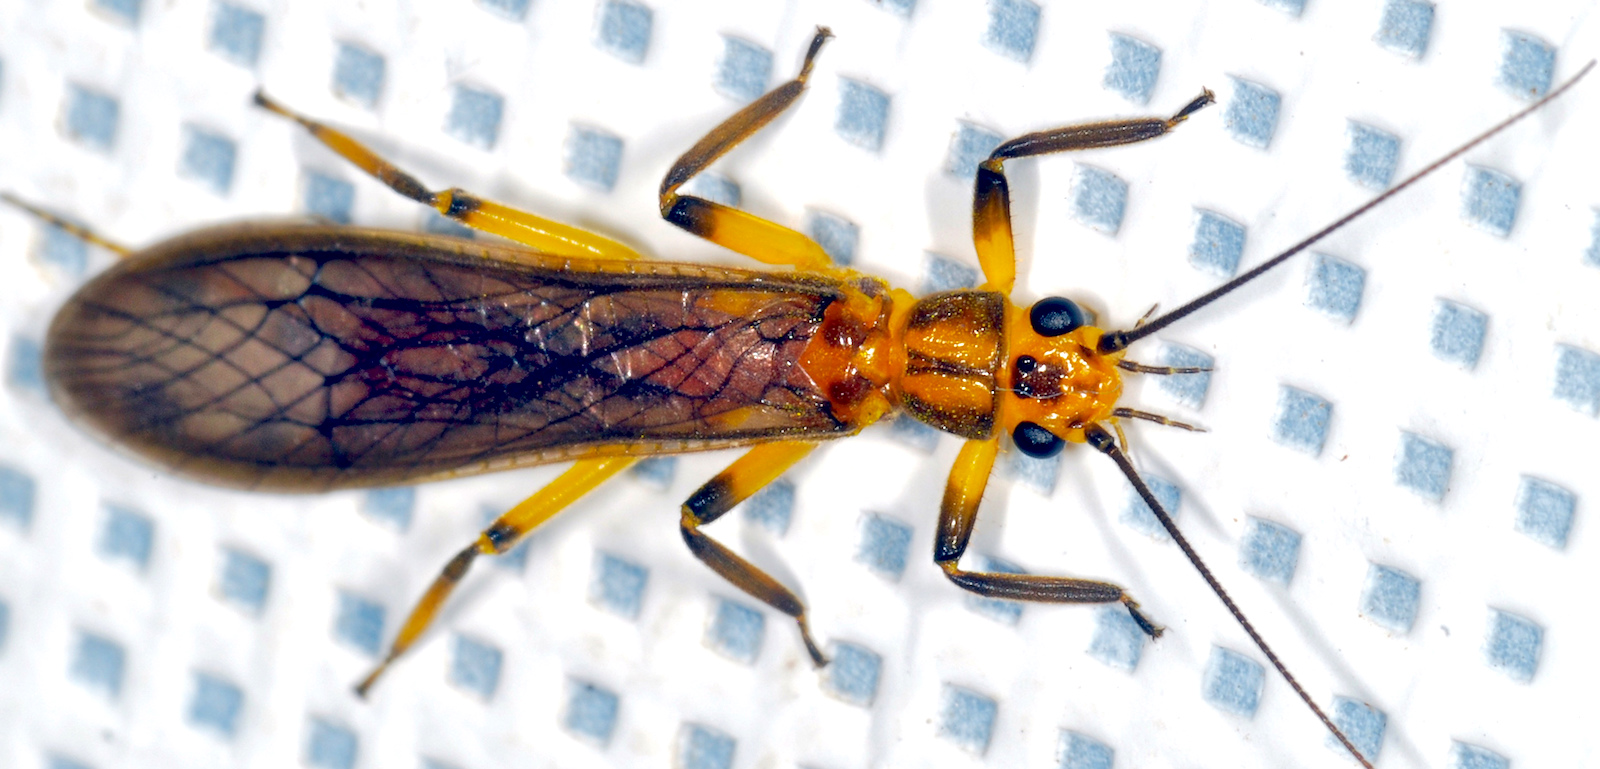
\includegraphics[width=0.45\textwidth]{Plecoptera}
\end{SCfigure}

\clearpage

\begin{SCfigure}[][ht!]
  \caption*{\textbf{Thysanoptera} (thrips). \textit{Habitat:} On leaves, flowers, under fallen logs. \textit{Collecting method:} Aspirator, net, Winkler extractor, Berlese funnel. \textit{How to euthanize:} Submerge in ethanol. \textit{Prepare specimens:} Normally slide-mounted but can be preserved in vials with ethanol (\textgreater70\%).\\ Photo: Katja Schulz (CC BY 2.0) \url{https://flic.kr/p/q6LxBS}}
  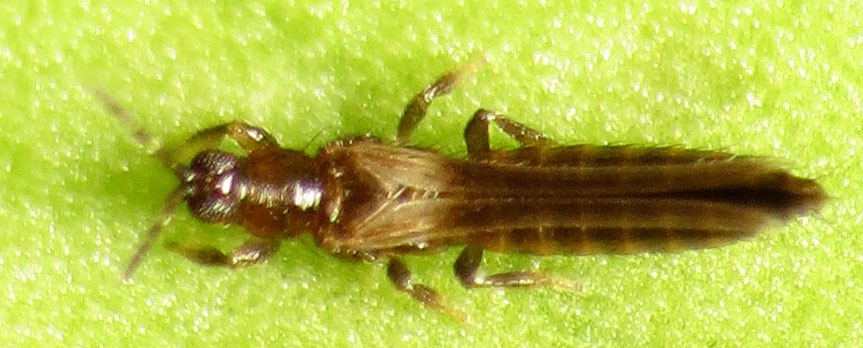
\includegraphics[width=0.45\textwidth]{Thysanoptera}
\end{SCfigure}

\begin{SCfigure}[][ht!]
  \caption*{\textbf{Psocodea} (bark lice, book lice, parasitic lice). \textit{Habitat:} On leaves and trunks, around books; parasitic species on mammals and birds. \textit{Collecting method:} Aspirator, forceps. \textit{How to euthanize:} Submerge in ethanol. \textit{Prepare specimens:} Normally slide-mounted but can be preserved in vials with ethanol (\textgreater70\%).\\ Photo: Ken Schneider (CC BY-NC 2.0) \url{https://flic.kr/p/mX6h9D}}
  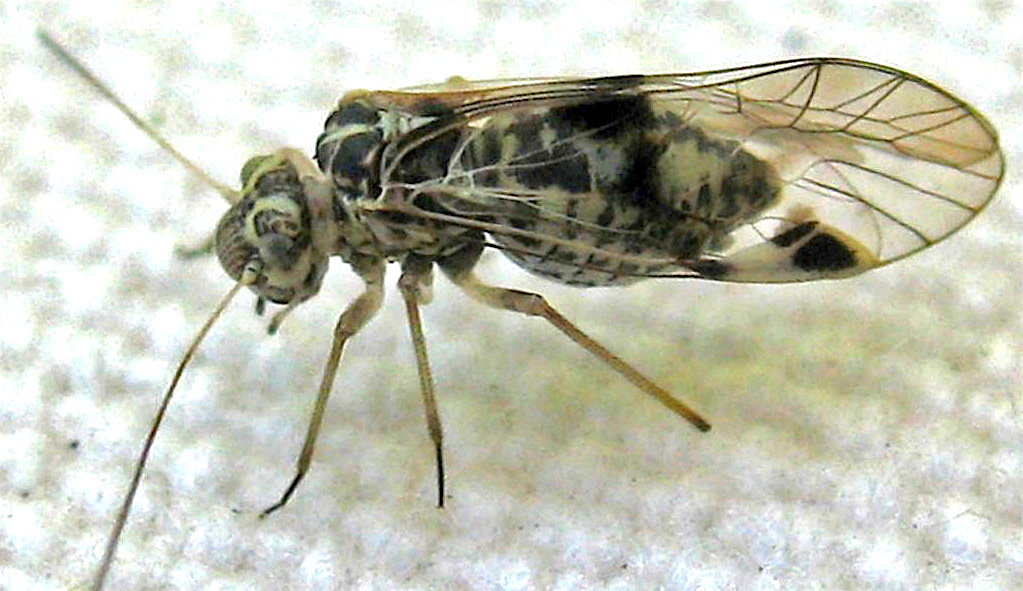
\includegraphics[width=0.45\textwidth]{PsocodeaBark}
\end{SCfigure}

\begin{SCfigure}[][ht!]
  \caption*{\textbf{Hemiptera: Heteroptera, Auchenorrhyncha} (true bugs, hoppers, cicadas). \textit{Habitat:} On plants, under logs, in/on water, on host mammals and birds; diverse and nearly ubiquitous. \textit{Collecting method:} Almost any method, depending on habitat targeted. \textit{How to euthanize:} Freeze, submerge in ethanol, or use kill jar with ethyl acetate. \textit{Prepare specimens:} Nymphs preserved in vials with ethanol (\textgreater70\%). Adults of most species are pinned through thorax, dorsal to mesothoracic legs. Note that wing venation, mouthparts, and antennae are important for family-level diagnosis.\\ Photo: NY State IPM Program (CC BY 2.0) \url{https://flic.kr/p/guTgFA}}
  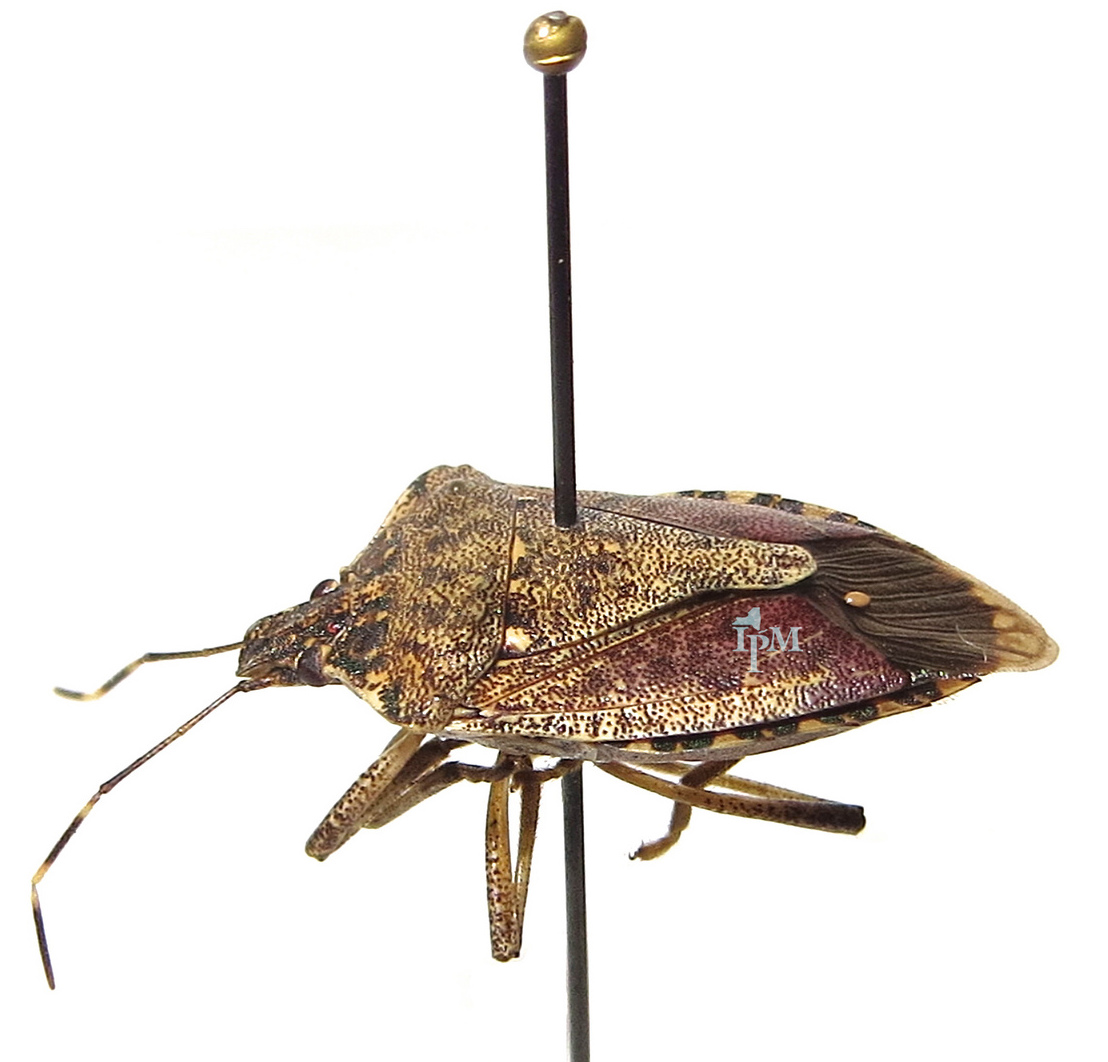
\includegraphics[width=0.45\textwidth]{HemipteraHeteroptera}
\end{SCfigure}

\clearpage

\begin{SCfigure}[][ht!]
  \caption*{\textbf{Hemiptera: Sternorrhyncha} (scale insects, aphids). \textit{Habitat:} On plants, especially leaves and stems \textit{Collecting method:} Aspirator, by hand. \textit{How to euthanize:} Freeze, submerge in ethanol. \textit{Prepare specimens:} Usually slide-mounted but can be preserved in vials with ethanol (\textgreater70\%).\\ Photo: Jon Sullivan (CC BY-NC 2.0) \url{https://flic.kr/p/oSAp1Y}}
  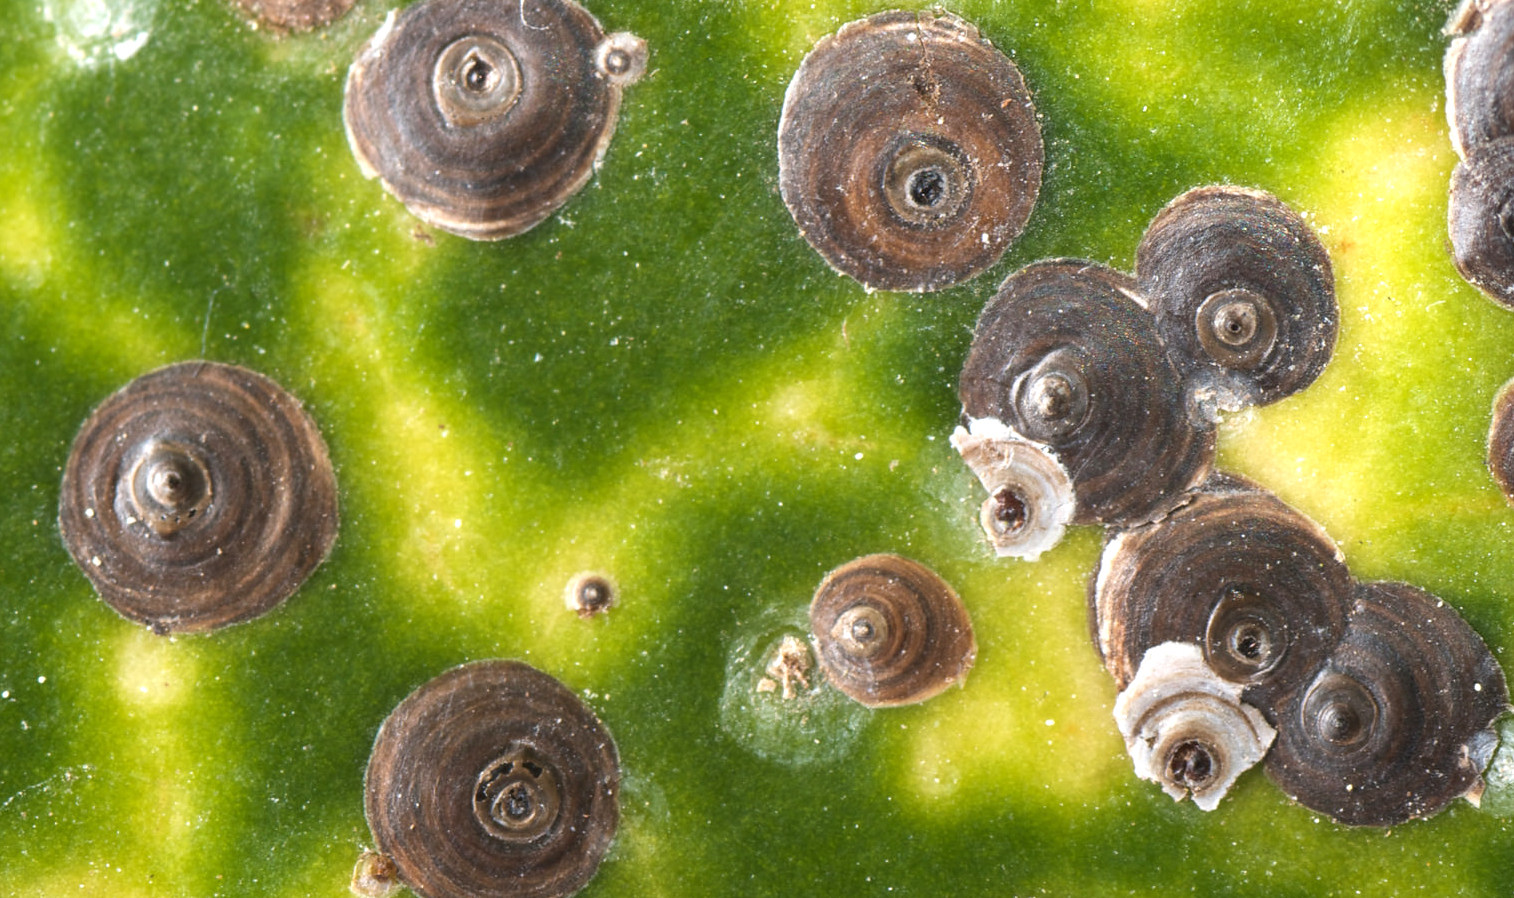
\includegraphics[width=0.45\textwidth]{HemipteraSternorrhyncha}
\end{SCfigure}

\begin{SCfigure}[][ht!]
  \caption*{\textbf{Mecoptera} (scorpionflies). \textit{Habitat:} On plants, on snow near trees. \textit{Collecting method:} Sweep net/aspirator, by hand, Malaise trap. \textit{How to euthanize:} Freeze, submerge in ethanol, or use kill jar with ethyl acetate. \textit{Prepare specimens:} Larvae and all Boreidae are preserved in vials with ethanol (\textgreater70\%). Adults are pinned through mesothorax.\\ Photo: Orest Shvadchak (CC BY-SA 2.0) \url{https://flic.kr/p/945m9F}}
  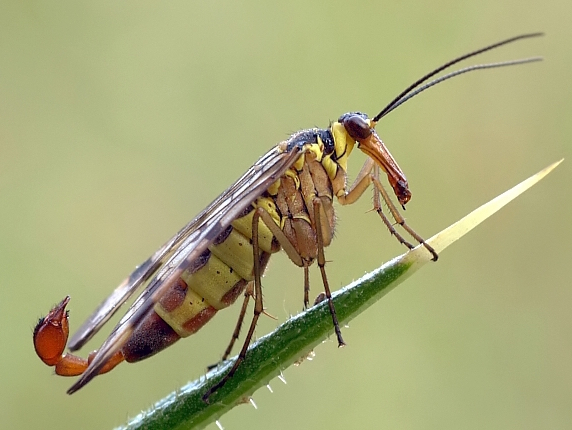
\includegraphics[width=0.45\textwidth]{Mecoptera}
\end{SCfigure}

\begin{SCfigure}[][ht!]
  \caption*{\textbf{Siphonaptera} (fleas). \textit{Habitat:} Larvae live in nests of their hosts. Adults usually found on host mammals and birds. \textit{Collecting method:} Aspirator, forceps. \textit{How to euthanize:} Submerge in ethanol. \textit{Prepare specimens:} Normally slide-mounted but can be preserved in vials with ethanol (\textgreater70\%).\\ Photo: AFPMB (CC0) \url{https://flic.kr/p/9bKUYn}}
  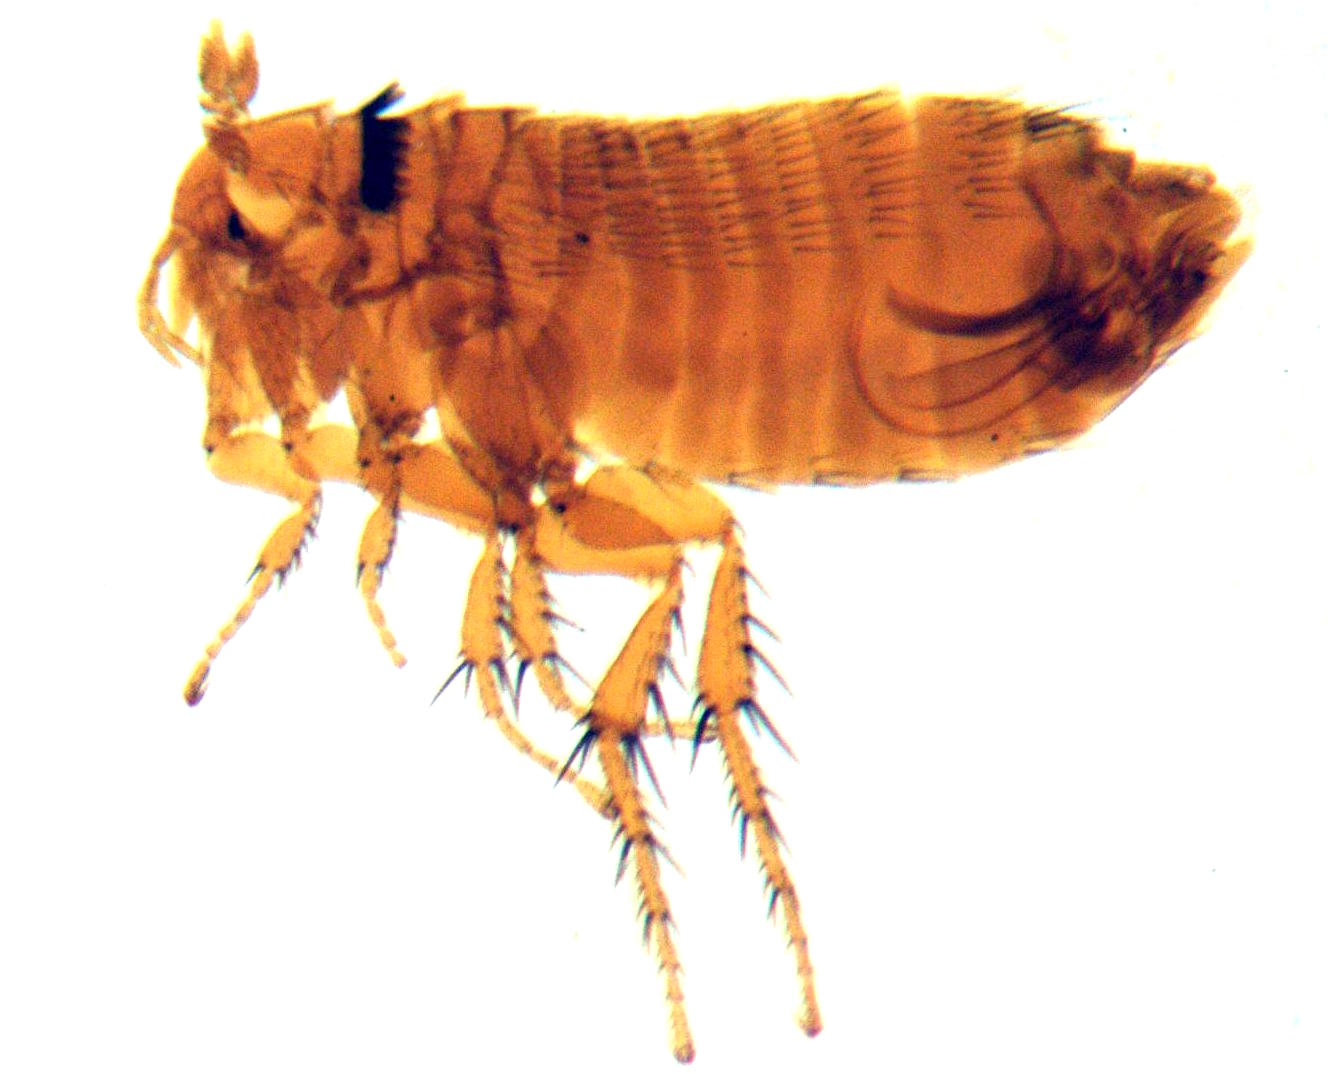
\includegraphics[width=0.45\textwidth]{Siphonaptera}
\end{SCfigure}

\clearpage

\begin{SCfigure}[][ht!]
  \caption*{\textbf{Diptera} (flies, gnats, mosquitoes). \textit{Habitat:} Diverse and nearly ubiquitous in most habitats. \textit{Collecting method:} Almost any method, depending on habitat targeted. Malaise traps and yellow bowls are especially effective for adults. \textit{How to euthanize:} Freeze, submerge in ethanol, or use kill jar with ethyl acetate. \textit{Prepare specimens:} Larvae and soft-bodied adults (\textit{e.g.}, Cecidomyiidae) preserved in vials with ethanol (\textgreater70\%). Adults of most species are pinned through thorax, dorsal to mesothoracic legs, or pointed dextrally. Adults should be pinned/pointed in a way that one can view all sclerites (\textit{i.e.}, legs away from body). Wing veins and bristle patterns are important for diagnosis. Also, scaly flies, like mosquitoes, should be double-mounted, with the minuten entering the thorax dextrally.\\ Photo: Troup Dresser (CC BY-NC 2.0) \url{https://flic.kr/p/cYaAPo}}
  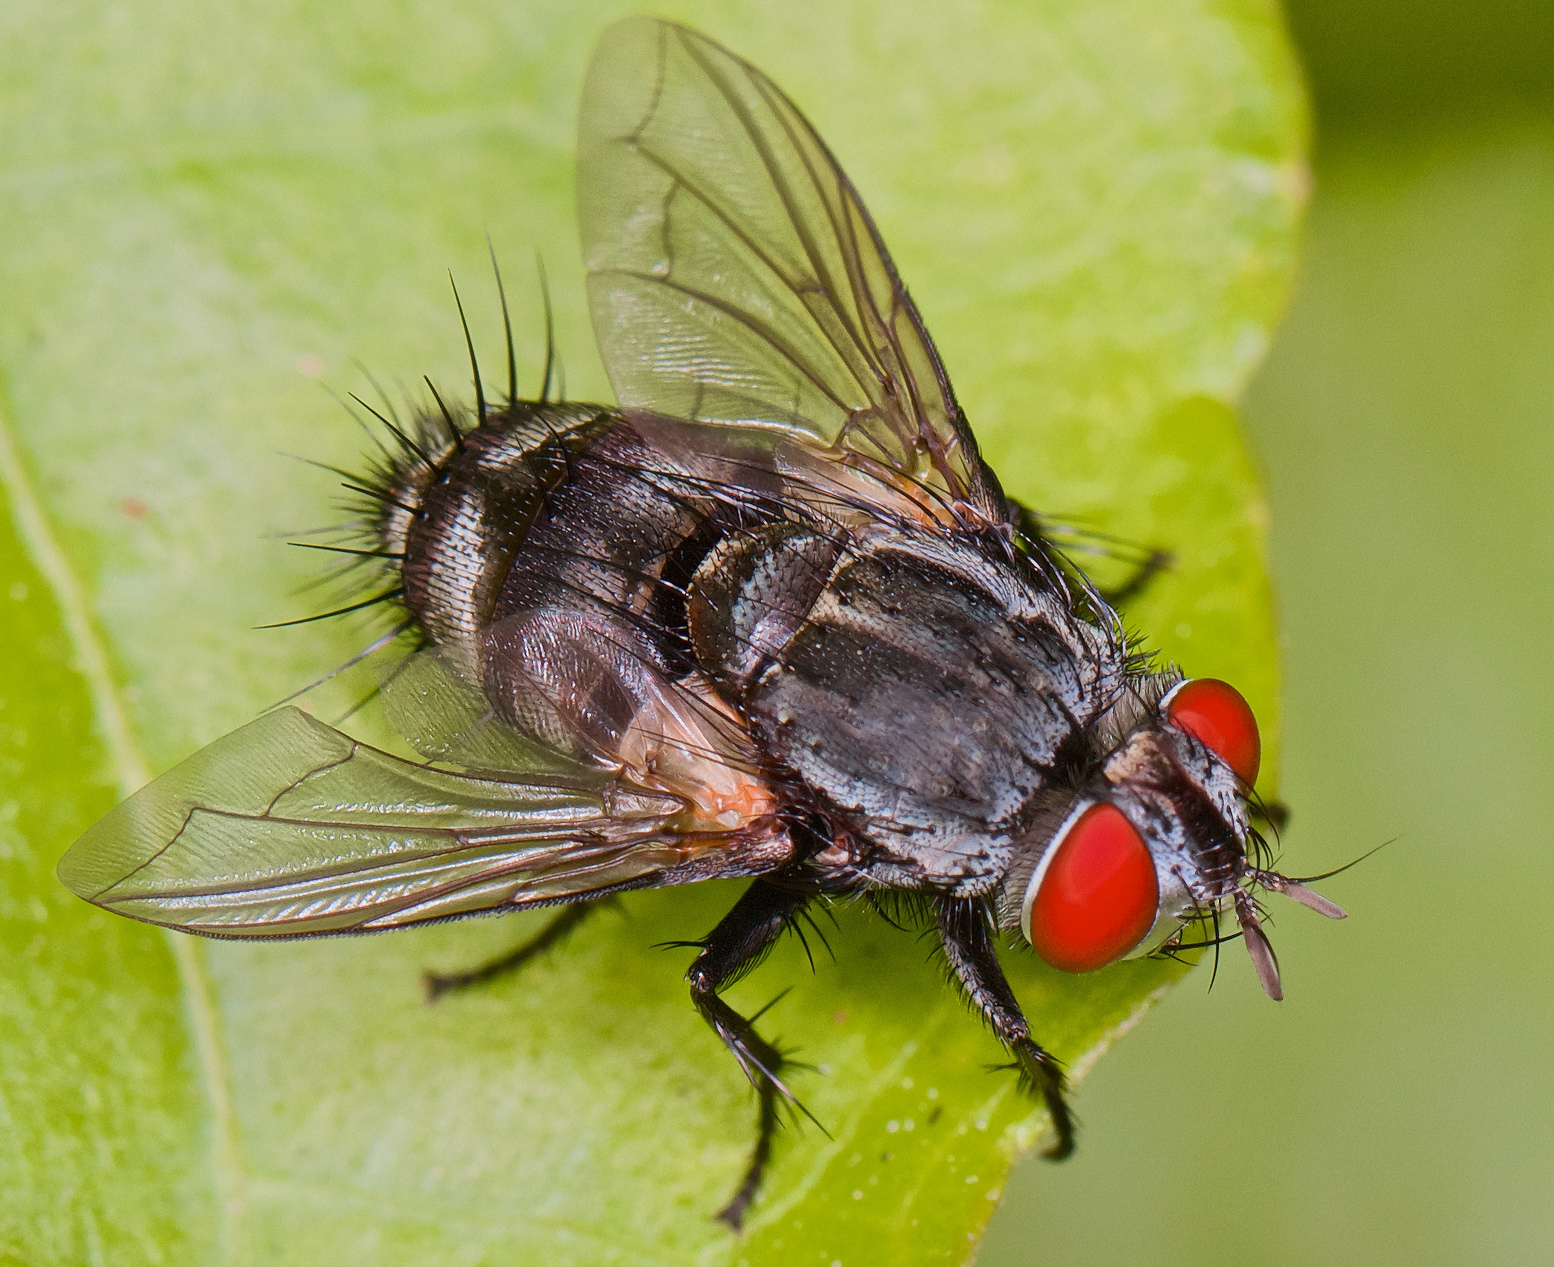
\includegraphics[width=0.45\textwidth]{Diptera}
\end{SCfigure}

\begin{SCfigure}[][ht!]
  \caption*{\textbf{Lepidoptera} (moths, butterflies). \textit{Habitat:} Diverse and nearly ubiquitous in most habitats. \textit{Collecting method:} Almost any method, depending on habitat targeted. Lights and baits are especially effective at luring adults adults. \textit{How to euthanize:} Freeze or use kill jar with ethyl acetate. \textit{Prepare specimens:} Larvae are preserved in vials with ethanol (\textgreater70\%). Adults of most species are pinned medially through thorax, dorsal to mesothoracic legs. Small specimens should be double-mounted, with minuten entering thorax similar to a normal pin. Wings of all specimens must be spread. \\ Photo: Andy Reago \& Chrissy McClarren (CC BY 2.0) \url{https://flic.kr/p/ofEZW6}}
  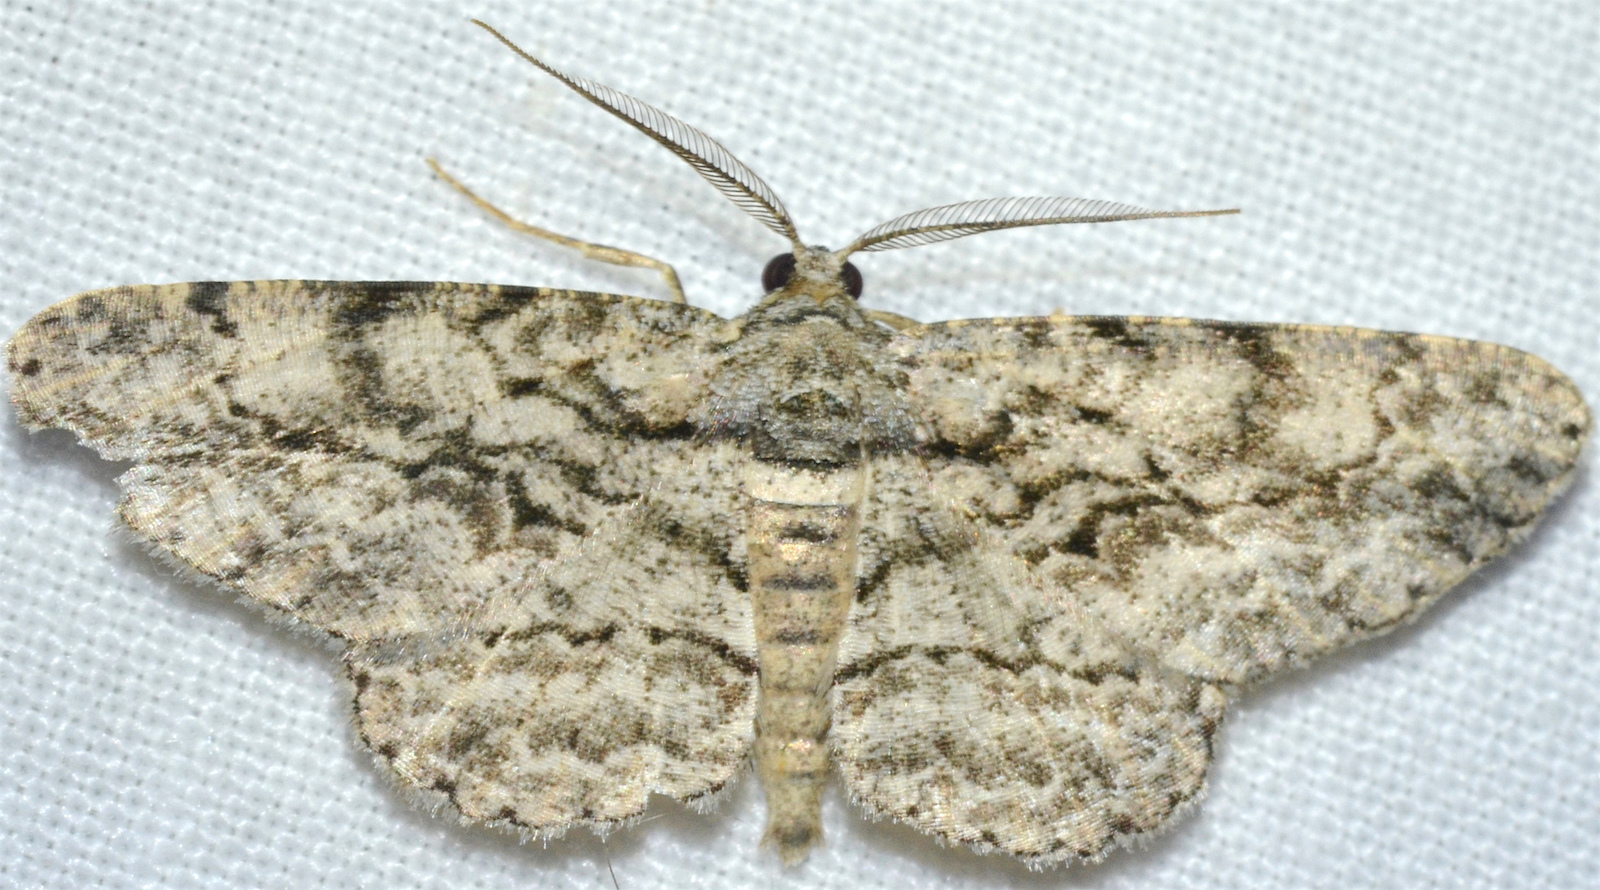
\includegraphics[width=0.45\textwidth]{Lepidoptera}
\end{SCfigure}

\begin{SCfigure}[][ht!]
  \caption*{\textbf{Trichoptera} (caddisflies). \textit{Habitat:} Immatures are aquatic; adults fly. \textit{Collecting method:} Use D-net for immatures; aspirator, net, and/or sheet at light for adults. \textit{How to euthanize:} Submerge in ethanol. \textit{Prepare specimens:} Preserve all stages in vials with ethanol (\textgreater70\%)\\ Photo: Macroscopic Solutions (CC BY-NC 2.0) \url{https://flic.kr/p/o4e7U7}}
  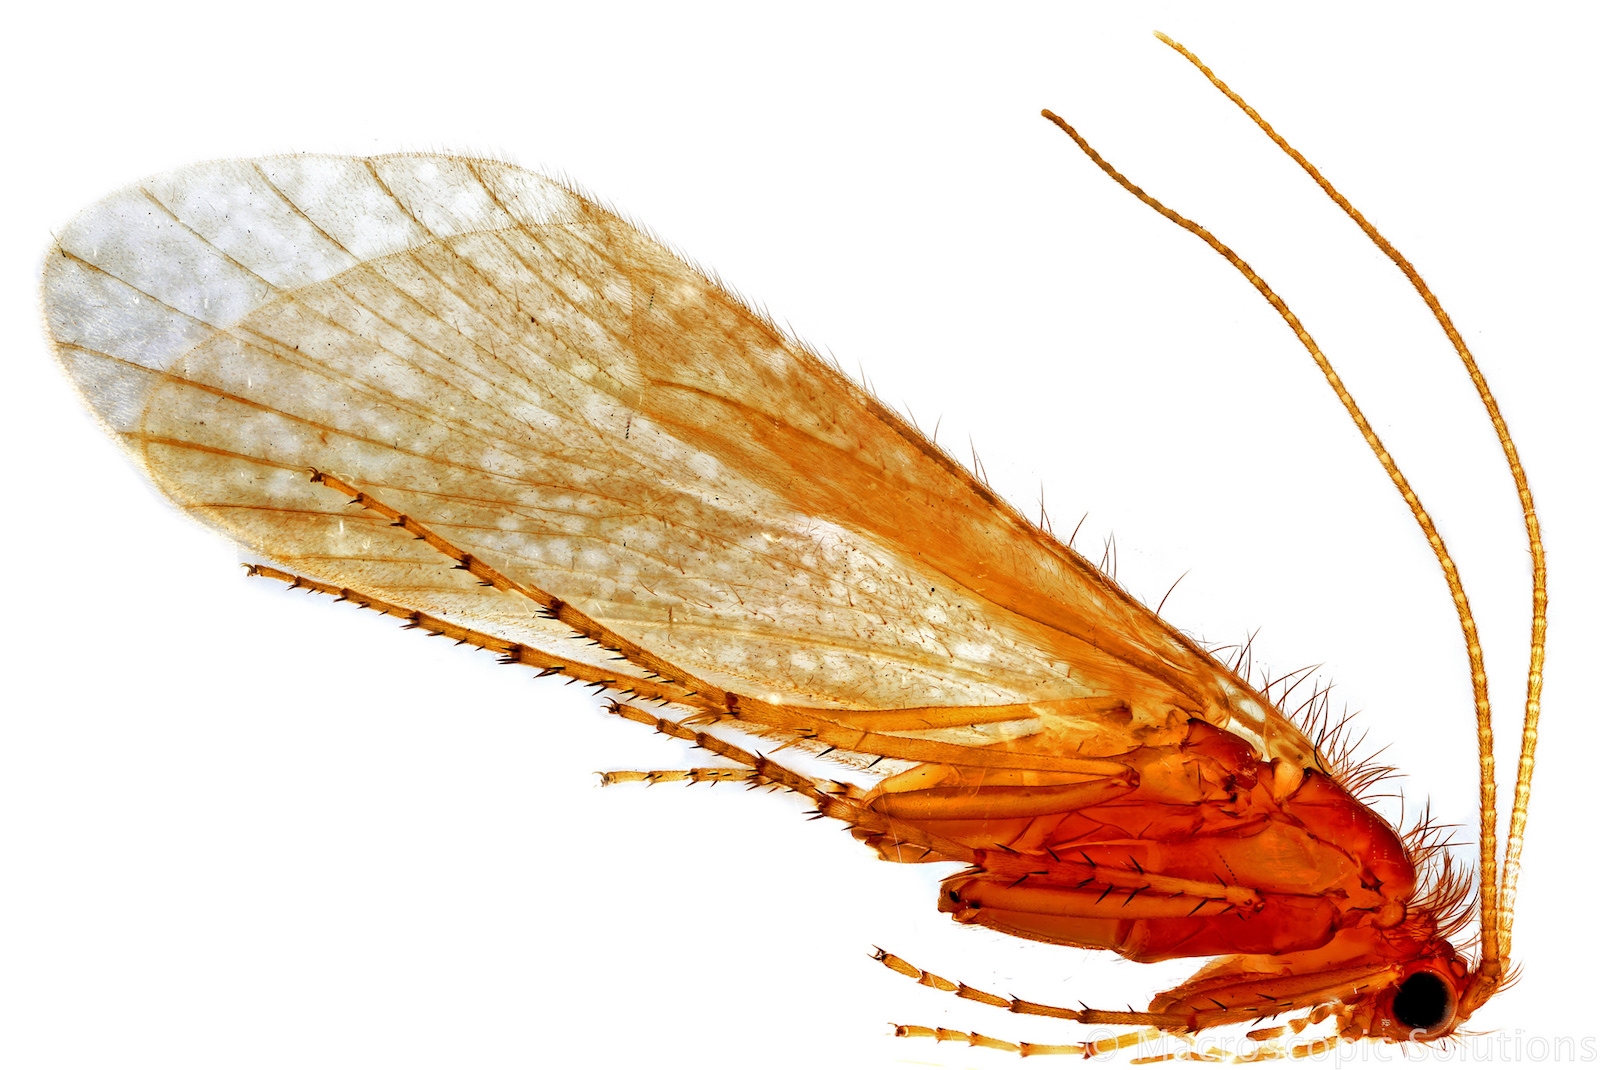
\includegraphics[width=0.45\textwidth]{Trichoptera}
\end{SCfigure}

\clearpage

\begin{SCfigure}[][ht!]
  \caption*{\textbf{Neuroptera} (lacewings, antlions, mantisflies).
  \textit{Habitat:} Immatures are terrestrial or aquatic; adults fly. \textit{Collecting method:} Aspirator, net, and/or sheet at light for adults. \textit{How to euthanize:} Submerge in ethanol, freeze, or use kill jar with ethyl acetate. \textit{Prepare specimens:} Larvae go in vials with ethanol (\textgreater70\%). Adults are pinned through the mesothorax and positioned in a way that minimizes their size (legs and antennae close to body).\\ Photo: Mick E. Talbot (CC BY 2.0) \url{https://flic.kr/p/6mWUDw}}
  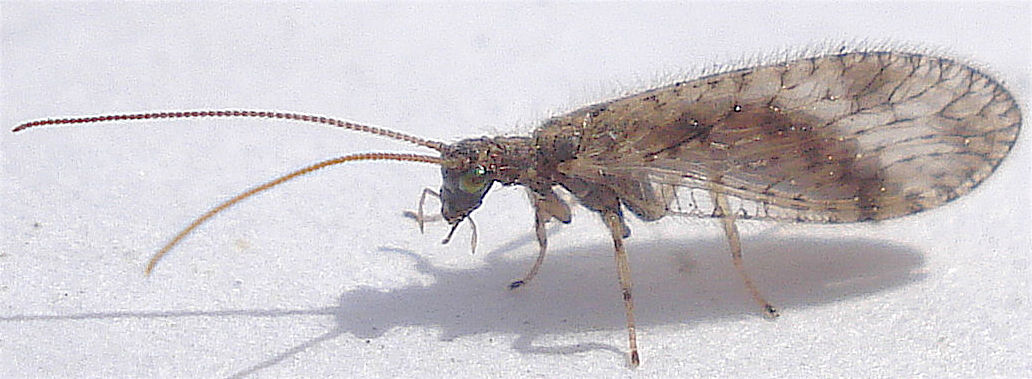
\includegraphics[width=0.45\textwidth]{Neuroptera}
\end{SCfigure}

\begin{SCfigure}[][ht!]
  \caption*{\textbf{Megaloptera} (dobsonflies, fishflies, alderflies). \textit{Habitat:} Immatures are aquatic; adults fly. \textit{Collecting method:} D-net for larvae; forceps, net, and/or sheet at light for adults. \textit{How to euthanize:} Submerge in ethanol (especially larvae), freeze, or use kill jar with ethyl acetate. \textit{Prepare specimens:} Larvae go in vials with ethanol (\textgreater70\%). Adults are pinned through the mesothorax and positioned in a way that minimizes their size (legs and antennae close to body).\\ Photo: Ronald Orosz (CC BY-NC 2.0) \url{https://flic.kr/p/4TEtzq}}
  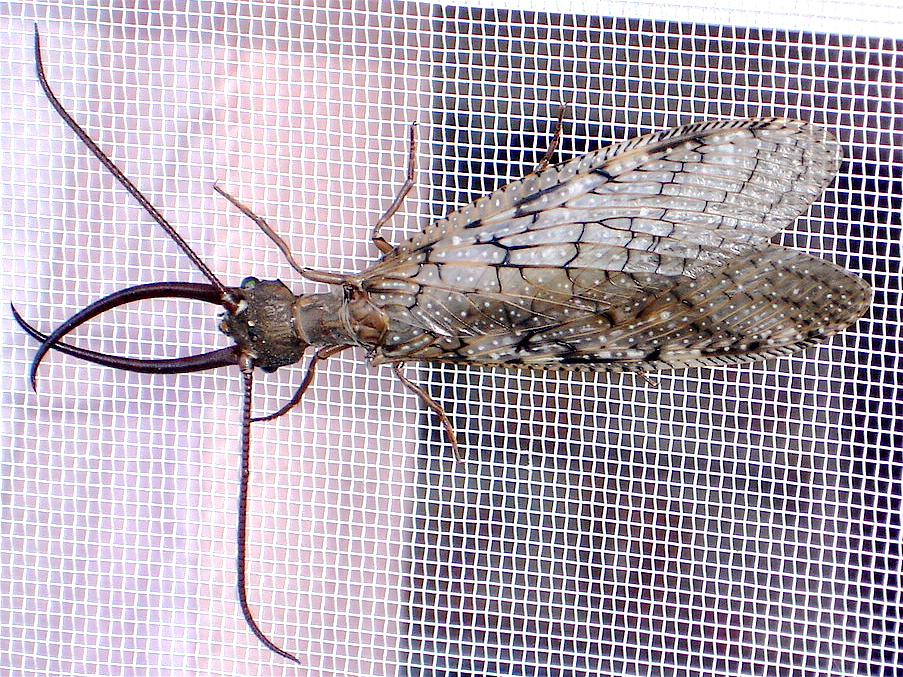
\includegraphics[width=0.45\textwidth]{Megaloptera}
\end{SCfigure}

\begin{SCfigure}[][ht!]
  \caption*{\textbf{Raphidioptera} (snakeflies). \textit{Habitat:} Larvae and adults are frequently associated with trees; in the USA they're found exclusively in the west. \textit{Collecting method:} Forceps, net. \textit{How to euthanize:} Submerge in ethanol (especially larvae), freeze, or use kill jar with ethyl acetate. \textit{Prepare specimens:} Larvae go in vials with ethanol (\textgreater70\%). Adults are pinned through the mesothorax and positioned in a way that minimizes their size (legs and antennae close to body).\\ Photo: Tab Tannery (CC BY-NC-SA 2.0) \url{https://flic.kr/p/92UMz6}}
  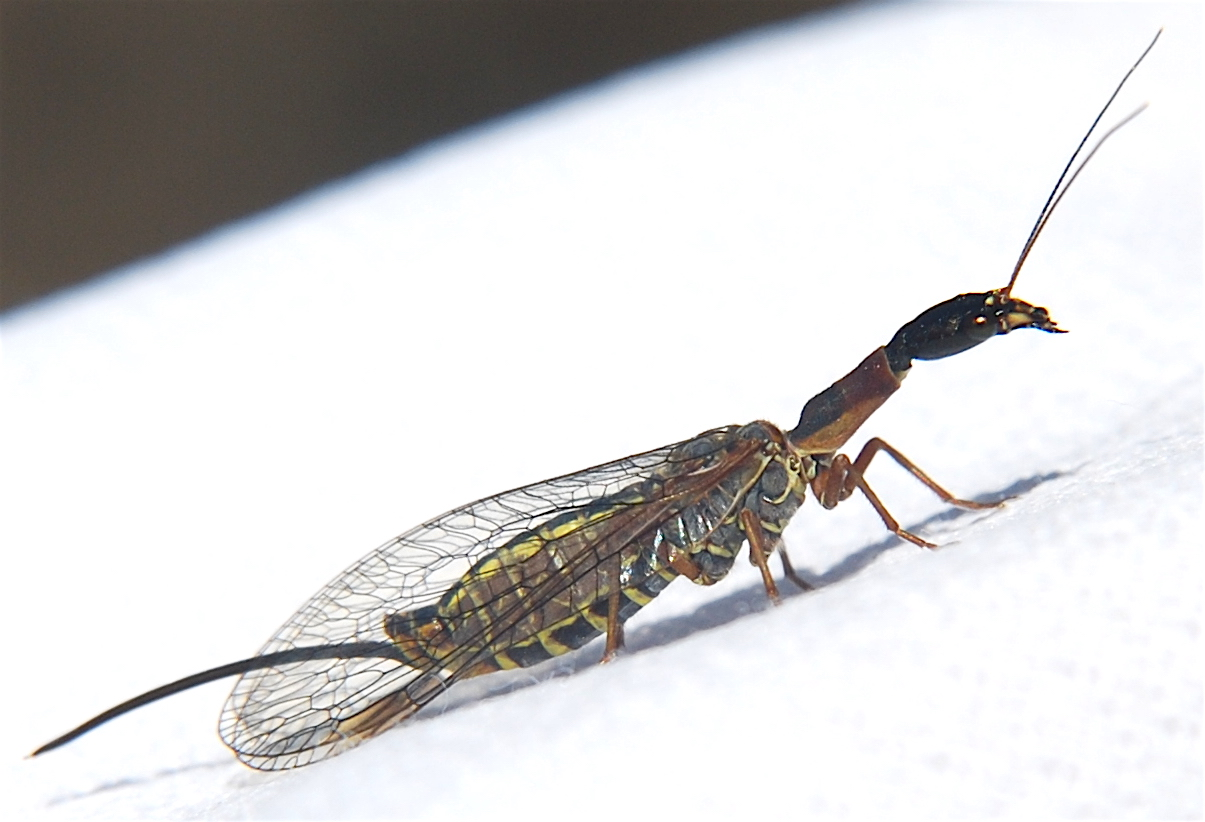
\includegraphics[width=0.45\textwidth]{Raphidioptera}
\end{SCfigure}

\clearpage

\begin{SCfigure}[][ht!]
  \caption*{\textbf{Strepsiptera} (twisted-wing parasites).\textit{Habitat:} Larvae, pupae, and adult females are usually found with their hosts (\textit{e.g.}, aculeate Hymenoptera, many hemipterans). \textit{Collecting method:} Malaise traps sometimes get males; other methods haphazardly collect these insects by collecting their hosts. \textit{How to euthanize:} Submerge in ethanol or use kill jar with ethyl acetate. \textit{Prepare specimens:} All stages go in vials with ethanol (\textgreater70\%). \\ Image: J. Sowerby (CC0), via Biodiversity Heritage Library \url{https://flic.kr/p/a9W5Qa}}
  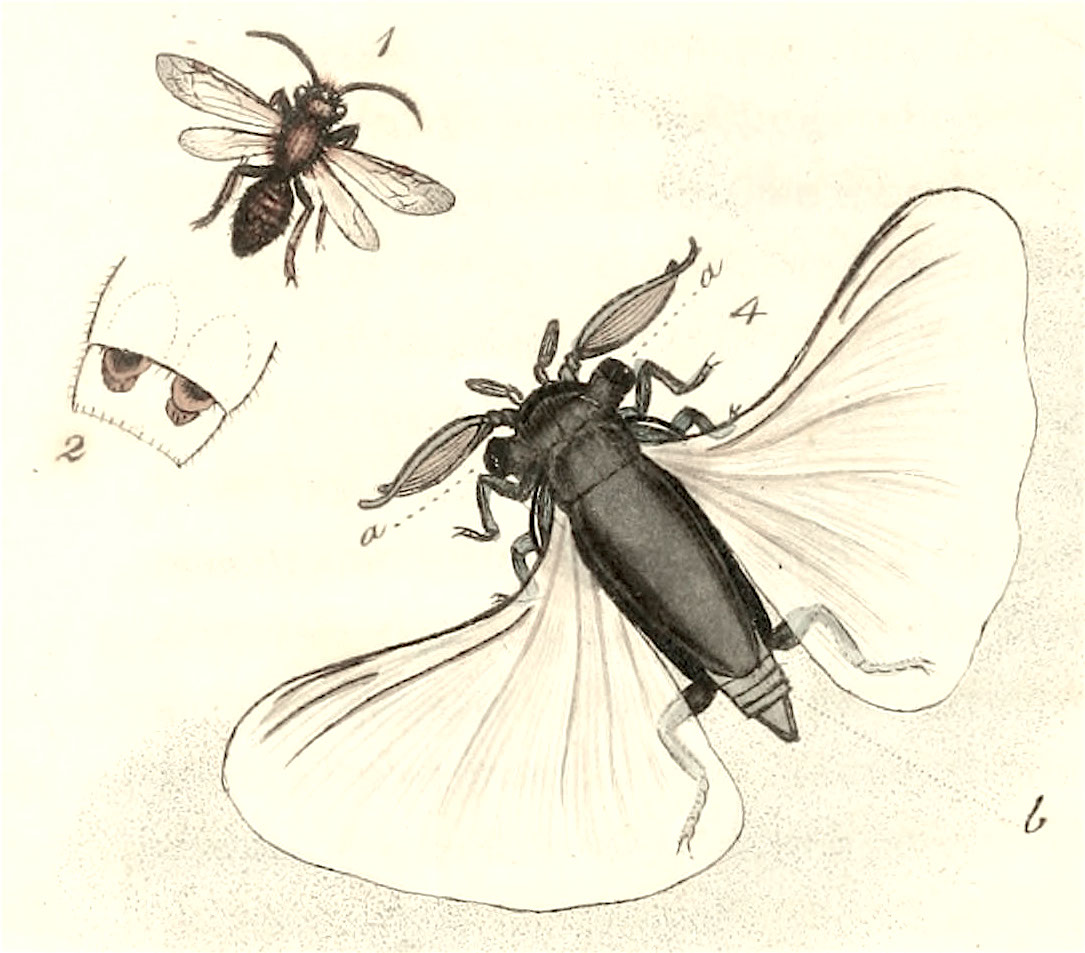
\includegraphics[width=0.45\textwidth]{Strepsiptera}
\end{SCfigure}

\begin{SCfigure}[][ht!]
  \caption*{\textbf{Coleoptera} (beetles). 
  \textit{Habitat:} Diverse and nearly ubiquitous in most habitats. \textit{Collecting method:} Almost any method, depending on habitat targeted. \textit{How to euthanize:} Freeze, submerge in ethanol, or use kill jar with ethyl acetate. \textit{Prepare specimens:} Larvae preserved in vials with ethanol (\textgreater70\%). Adults are pinned through right elytron, dorsal to mesothoracic legs, or pointed dextrally. Adults should be pinned/pointed in a way that one can view antennae, all legs, and the ventral sclerites. \\ Photo: Gilles San Martin (CC BY-SA 2.0) \url{https://flic.kr/p/hCtNmf}}
  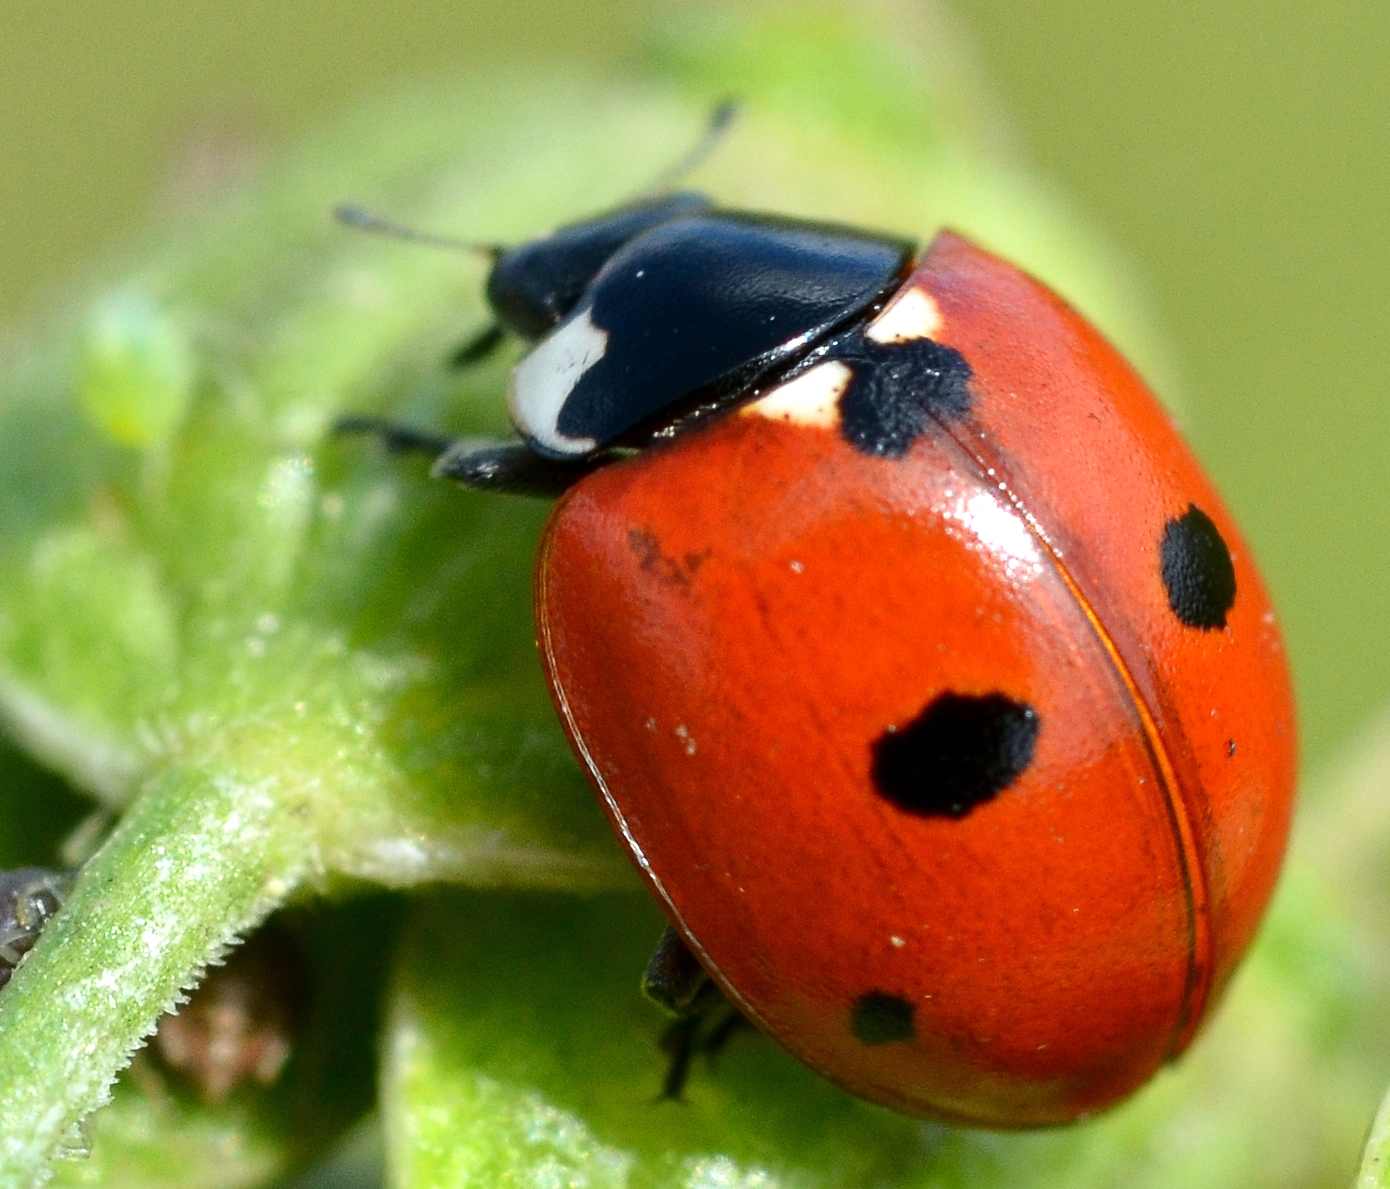
\includegraphics[width=0.45\textwidth]{Coleoptera}
\end{SCfigure}

\begin{SCfigure}[][ht!]
  \caption*{\textbf{Hymenoptera} (sawflies, wasps, ants, bees).   \textit{Habitat:} Diverse and nearly ubiquitous in most habitats. \textit{Collecting method:} Almost any method, depending on habitat targeted, but yellow bowls and Malaise traps are especially effective. \textit{How to euthanize:} Freeze, submerge in ethanol, or use kill jar with ethyl acetate. \textit{Prepare specimens:} Adults are pinned through mesothorax, dorsal to mesothoracic legs, or pointed dextrally. Head characters, wing venation, and ventral sclerite morphology can be important for family-level diagnosis. Small, dainty hymenopterans with soft cuticle (e.g., most Chalcidoidea) and larvae should be preserved in vials with ethanol  (\textgreater70\%).\\ Photo: Patrick\_K59 (CC BY 2.0) \url{https://flic.kr/p/peXyQ8}}
  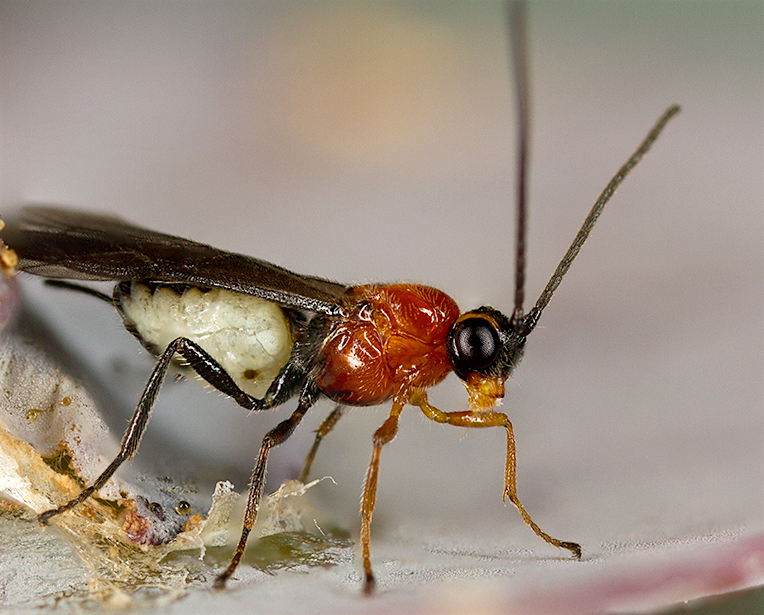
\includegraphics[width=0.45\textwidth]{Hymenoptera}
\end{SCfigure}

\end{document}
